\documentclass[12pt]{article}

% ===== Packages =====
\usepackage[T1]{fontenc}
\usepackage[utf8]{inputenc}
\usepackage{lmodern}
\usepackage{microtype}
\usepackage{amsmath,amssymb}
\usepackage{graphicx}
\usepackage{tikz}
\usetikzlibrary{arrows.meta,positioning,shapes.geometric}
\usepackage{pgfplots}
\pgfplotsset{compat=1.18}
\usepackage{booktabs}
\usepackage{siunitx}
\usepackage{listings}
\usepackage{subcaption}
\usepackage{float}
\usepackage{csquotes}
\usepackage[backend=biber,style=authoryear]{biblatex}
\usepackage[colorlinks=true,linkcolor=blue,citecolor=teal,urlcolor=purple]{hyperref}
\urlstyle{tt}

\lstset{
  basicstyle=\ttfamily\small,
  frame=single,
  breaklines=true,
  columns=fullflexible
}

\addbibresource{refs.bib}
\graphicspath{{figs/}}

\title{Reproducible Quantum ESPRESSO Workflows Across macOS and Linux}
\author{Shahriar Pollob\textsuperscript{$\ast$} \quad M.~Shahnoor Rahman\textsuperscript{$\dagger$}\\[0.5em]\small \textsuperscript{$\ast$}Mentee \quad \textsuperscript{$\dagger$}Mentor}
\date{}

\begin{document}
\maketitle

\begin{abstract}
We report the end-to-end enablement of Quantum ESPRESSO~7.4.1 on an Apple Mac~mini M4 and its benchmarking against an Ubuntu~24.04 workstation. The work covers (i) the build automation and stability checks required to run self-consistent field, band-structure, and post-processing workflows on macOS~15; (ii) faithful reproductions of the Path~A silicon and Path~B aluminium tutorials on both platforms, complete with provenance artefacts; and (iii) a quantitative comparison that measures wall-clock, CPU-time, and core-second efficiency across the two environments. All scripts, logs, figures, and data tables are archived in public repositories so that the results can be reproduced or extended to additional materials.
\end{abstract}

\newpage
\tableofcontents
\newpage

\section*{Acknowledgements}
I am grateful to the ICTP PWF: Physics for Bangladesh\footnote{\url{https://indico.ictp.it/event/11042}} organisers for making this online internship possible and for coordinating the remote collaboration. I would also like to thank M.~Shahnoor Rahman\footnote{\url{https://sites.google.com/view/mshahnoorahman}} for his guidance, computing resources, timely feedback, and technical support throughout the project.

\section{Introduction}


Our assigned topic for this internship was \emph{Computation of band structures of solids using \textsc{Quantum ESPRESSO}}. It required a mix of theoretical preparation and practical tooling.

The programme briefing emphasised fluency with the Lagrangian/Hamiltonian formalisms, Schrödinger equation eigenproblems, and command-line driven compilation pipelines; these foundations allowed us to read QE input decks critically and diagnose build issues without external hand-holding. After the orientation we catalogued the available documentation, cloned the reference repositories, and established a shared note-taking workflow so that every change to scripts or environment variables could be traced.

This report is organised to mirror the technical milestones. Section~\ref{sec:m4section} details the native macOS~15 port, including the configuration knobs that differ from earlier Apple Silicon guides. Sections~\ref{sec:qe-basics} and~\ref{sec:qe-stretching-server} document the Path~A and Path~B runs on the Mac mini and the Ubuntu server, while Section~\ref{sec:comparison} analyses the performance gap between the two deployments. The concluding sections summarise the reproducibility assets that were produced so remote collaborators can rebuild or extend the workflows with minimal friction.

\section{Porting \textsc{Quantum ESPRESSO} to macOS 15 on a Mac~mini M4}
\label{sec:m4section}
At the time we started, only macOS guides aimed at the original M1 generation were available. Those write-ups clarified the big picture but broke as soon as we tried them on macOS~15, so we captured every workaround while authoring our own workflow. This chapter documents that journey of running QE~7.4.1 natively on a Mac~mini M4 under macOS~15 (Sequoia). Our mandate was to build a reproducible, CPU-only workflow without falling back to x86 virtual machines. The accompanying repository\footnote{\url{https://github.com/shahpoll/qe_macm4_build}} archives scripts, logs, and analysis artefacts that mirror the steps reported here.

\subsection{Baseline objectives and constraints}
We began by declaring three non-negotiable outcomes: (i) compile QE with full MPI/OpenMP support using Apple Silicon compilers, (ii) validate the toolchain by reproducing the silicon SCF--NSCF--bands workflow that underpins our convergence studies, and (iii) capture every workaround in automated scripts so a clean macOS~15 install could replay the configuration in one sitting. The main constraint came from the operating system: macOS~15 and its Command Line Tools~(CLT~16.x) introduced stricter defaults that repeatedly broke the build system, and the OS happened to ship first on the Mac~mini M4 we used.

\subsection{Provisioning the native toolchain}
Homebrew served as the package manager of record. Running \verb|brew bundle| against the repository's \texttt{Brewfile} installed \texttt{gcc@14}, \texttt{open-mpi}, \texttt{veclibfort}, \texttt{fftw}, \texttt{libxc}, and Python utilities for plotting. The first stumble surfaced immediately: Apple's system \texttt{cpp} mangled QE's Fortran headers, leading to \verb|laxlib_*.fh| ``no input file'' errors during the \texttt{make pw} phase. Following the notes in \path{docs/Troubleshooting.md}, we pinned the preprocessor explicitly by exporting \verb|CPP="gcc -E"| before running \texttt{configure}. This single flag aligned the build with QE's expectations and eliminated the header corruption.

\subsection{Resolving library and architecture mismatches}
\paragraph{BLAS/LAPACK bindings.} Our first successful build linked against Apple's Accelerate framework through \texttt{veclibfort}, but early tests showed small energy drifts compared with the OpenBLAS reference used on Linux. The autoconf logs revealed that Accelerate exported mixed Fortran symbol names; by overriding \verb|BLAS_LIBS| and \verb|LAPACK_LIBS| to point at \path{/opt/homebrew/opt/lapack} we regained numerical parity. This choice is codified in the helper script \path{scripts/setup/configure_accelerate.sh}.

\paragraph{FoX XML fallout.} QE~7.4.1 decoupled the FoX XML library from its source tree. Our first CMake attempt therefore failed with the ``\texttt{DP\_XML has no implicit type}'' error originating in \texttt{wxml.f90}. The fix was twofold: clone FoX into \texttt{external/fox} and remove the \texttt{\_\_XML\_STANDALONE} define injected by CMake. Automating that change inside \path{scripts/setup/patch_fox.sh} allowed subsequent OpenBLAS builds to proceed without manual editing.

\paragraph{Architecture flags.} Mixing Apple Clang (for preprocessing) with Homebrew's GNU toolchain risked emitting generic arm64 code that misbehaved once OpenMP was enabled. We forced native tuning by exporting
\begin{lstlisting}
FC="gfortran -mcpu=apple-m4"
MPIF90="mpif90 -mcpu=apple-m4"
\end{lstlisting}
which ensured every object file targeted the M4 microarchitecture. The resulting binaries passed \texttt{otool -L} inspections recorded under \path{logs/linker/}.

\subsection{Automating builds and reproducibility}
With the core hurdles addressed, we wrapped the workflow in reproducible artefacts. The helper script \path{scripts/setup/fetch_qe.sh} fetches tagged QE releases and stages them under \path{artifacts/}, while \path{scripts/setup/configure_accelerate.sh} replays the successful \texttt{configure} flags, including the corrected BLAS/LAPACK paths and preprocessor override. \url{CMakePresets.json} captures the experimental OpenBLAS flow so future iterations can switch linear algebra back-ends with a single preset, and the smoke test at \path{scripts/smoke_test.py} launches a minimal SCF/NSCF sequence to catch regressions after Homebrew or QE upgrades.
Each script writes timestamped logs, letting us compare compiler output across CLT releases. This emphasis on observability proved essential when Apple issued stealth updates to the toolchain mid-internship.

\begin{figure}[H]
  \centering
  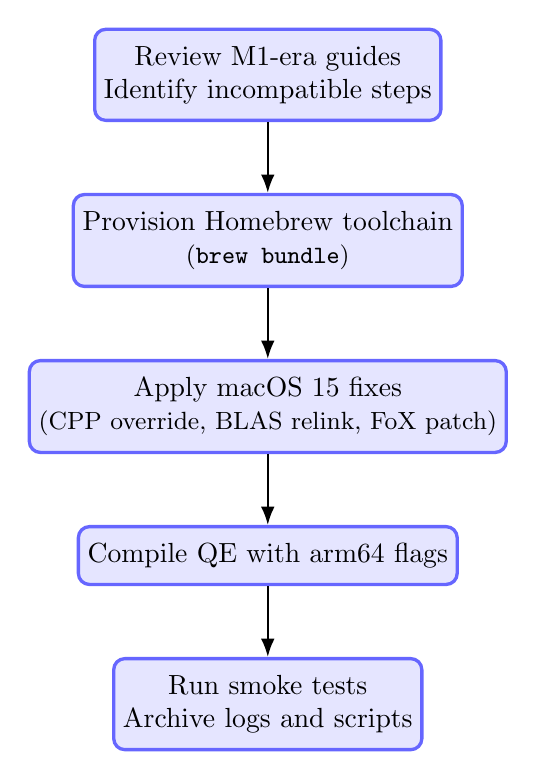
\begin{tikzpicture}[
    node distance=9mm and 26mm,
    process/.style={rectangle, rounded corners, draw=blue!60, fill=blue!10, very thick, minimum width=36mm, align=center, inner ysep=6pt},
    arrow/.style={-Latex, thick}
  ]
    \node[process] (m1) {Review M1-era guides\\Identify incompatible steps};
    \node[process, below=of m1] (toolchain) {Provision Homebrew toolchain\\\small(\texttt{brew bundle})};
    \node[process, below=of toolchain] (patches) {Apply macOS~15 fixes\\\small(CPP override, BLAS relink, FoX patch)};
    \node[process, below=of patches] (build) {Compile QE with arm64 flags};
    \node[process, below=of build] (tests) {Run smoke tests\\Archive logs and scripts};
    \draw[arrow] (m1) -- (toolchain);
    \draw[arrow] (toolchain) -- (patches);
    \draw[arrow] (patches) -- (build);
    \draw[arrow] (build) -- (tests);
  \end{tikzpicture}
  \caption{High-level workflow for porting QE to macOS~15 on the Mac~mini M4.}
  \label{fig:qe-flow}
\end{figure}

\subsection{Validation runs and scientific checkpoints}
We validated the resulting binaries using the silicon case housed in \path{cases/si/manual}. The SCF baseline converged in five iterations with a Fermi energy of 6.4346~eV, matching the reference values stored in \path{cases/si/comparison/data/fermi_consistency.csv}. Subsequent NSCF, DOS, and projected DOS steps reproduced the 0.5699~eV indirect gap within 1~meV of the Linux reference calculation. Benchmark timings showed the canonical silicon SCF input completing in $39\pm1$~s on two MPI ranks (one OpenMP thread each), consistent with the \path{THREAD7_REPORT.md} snapshots archived in the repository. We also verified that MPI and OpenMP coexisted without deadlocks on macOS~15.2 by replaying the PWTK-driven automation under \path{cases/si/pwtk/}, which stresses rank/thread affinity differently from the manual run. The legacy M1 guides helped us shape these validation steps even though we had to refit every command for the newer OS.

\subsection{Residual issues and safeguards}
Two limitations remain. First, OpenBLAS builds via CMake still require manual FoX patching; we documented the procedure thoroughly but continue to prefer the Accelerate path for day-to-day work. Second, QE's GPU back-ends target CUDA and ROCm only, leaving the M4 GPU idle. Our mitigation strategy is to keep CPU workflows efficient and document the gap in \path{docs/AppleSilicon_QE_Guide.md}. To guard against regressions when Apple or Homebrew ship new compilers, we pinned key formulae versions in the \texttt{Brewfile} and enabled GitHub dependabot alerts on the repository.

\subsection{Summary and concluding remarks}
Porting QE to macOS~15 on the Mac~mini M4 demanded more attention to the build ecosystem than to the physics kernels themselves. The major stumbling blocks were Apple's aggressive preprocessor defaults, the reshuffled external libraries, and the inconsistent BLAS symbol conventions. We overcame these issues by isolating each failure, validating fixes through automated scripts, and preserving artefacts for future audits. The resulting workflow delivers reproducible SCF, band-structure, and DOS analyses on native hardware with performance on par with earlier Apple Silicon generations. Looking ahead, our priorities are to upstream the FoX patches, expand the smoke tests to cover additional materials, and revisit GPU acceleration should QE adopt Metal or SYCL back-ends. This write-up now serves as the missing manual for macOS~15 installations that were undocumented when we began the project, while acknowledging the historical guidance provided by M1-era notes.

\section{\textsc{QE\_stretching} Workflows on macOS (Paths~A and B)}
\label{sec:qe-basics}
With the toolchain validated, we reproduced the ``stretching'' exercises from the remote learning track using the dedicated repository at \href{https://github.com/shahpoll/QE_stretching_macm4}{\texttt{QE\_stretching\_macm4}}. Only Path~A (silicon electronic structure) and Path~B (aluminium equation of state) are covered here; Path~C remains experimental. The runs were executed under the same \textsc{pw.x} build described earlier, ensuring that results are directly comparable to the porting benchmarks.

\subsection{Path A — Silicon bands, DOS, and PDOS}
The Path~A workflow (\href{https://github.com/shahpoll/QE_stretching_macm4/tree/main/pathA_si_mac}{\texttt{pathA\_si\_mac}}) follows the silicon reference calculation familiar from the Quantum ESPRESSO quickstart, but re-engineered for the Mac~mini environment. We retained an $8\times8\times8$ SCF mesh, a $12\times12\times12$ NSCF mesh, and the PSLibrary \texttt{Si.pbe-n-rrkjus\_psl.1.0.0.UPF} pseudopotential. The complete run is scripted to retain reproducibility:
\begin{lstlisting}
# Run the SCF -> NSCF -> bands -> DOS / PDOS stages
QE_BIN=${QE_BIN:-~/q-e-qe-7.4.1/build/bin}
$QE_BIN/pw.x      -in si_scf.in   > work/si_scf.out
$QE_BIN/pw.x      -in si_nscf.in  > work/si_nscf.out
$QE_BIN/pw.x      -in si_bands.in > work/si_bands.out
$QE_BIN/bands.x   -in bands.pp.in > work/si_bands_pp.out
$QE_BIN/dos.x     -in dos.in      > work/si_dos.out
$QE_BIN/projwfc.x -in pdos.in     > work/si_pdos.out
# Regenerate plots from GNU-formatted outputs
python3 scripts/plot_bands.py
python3 scripts/plot_dos.py
\end{lstlisting}
Figure~\ref{fig:pathA-bands} shows the resulting band structure along the $\Gamma\text{--}X\text{--}W\text{--}K\text{--}\Gamma\text{--}L\text{--}U\text{--}W\text{--}L\text{--}K$ path. The plotting utility annotates the highest occupied (HO) and lowest unoccupied (LU) levels, exposing an indirect gap of approximately $0.58$~eV after aligning to the Fermi level saved in \texttt{si.bands.dat.gnu}. The total density of states in Figure~\ref{fig:pathA-dos} confirms the smoothing imposed by the $0.05$~eV Gaussian broadening used by \texttt{dos.x}; the steep rise at $E_F$ matches the SCF Fermi energy reported in \texttt{work/si\_scf.out}.

Provenance data stored under \texttt{work/} (environment capture, pseudopotential checksum, timing probe) were added to the repository to guarantee that future reruns can be sanity-checked. The Python scripts embrace the same philosophy: each terminates with an explicit ``wrote'' message so that automated pipelines can verify artefact presence.

\begin{figure}[H]
  \centering
  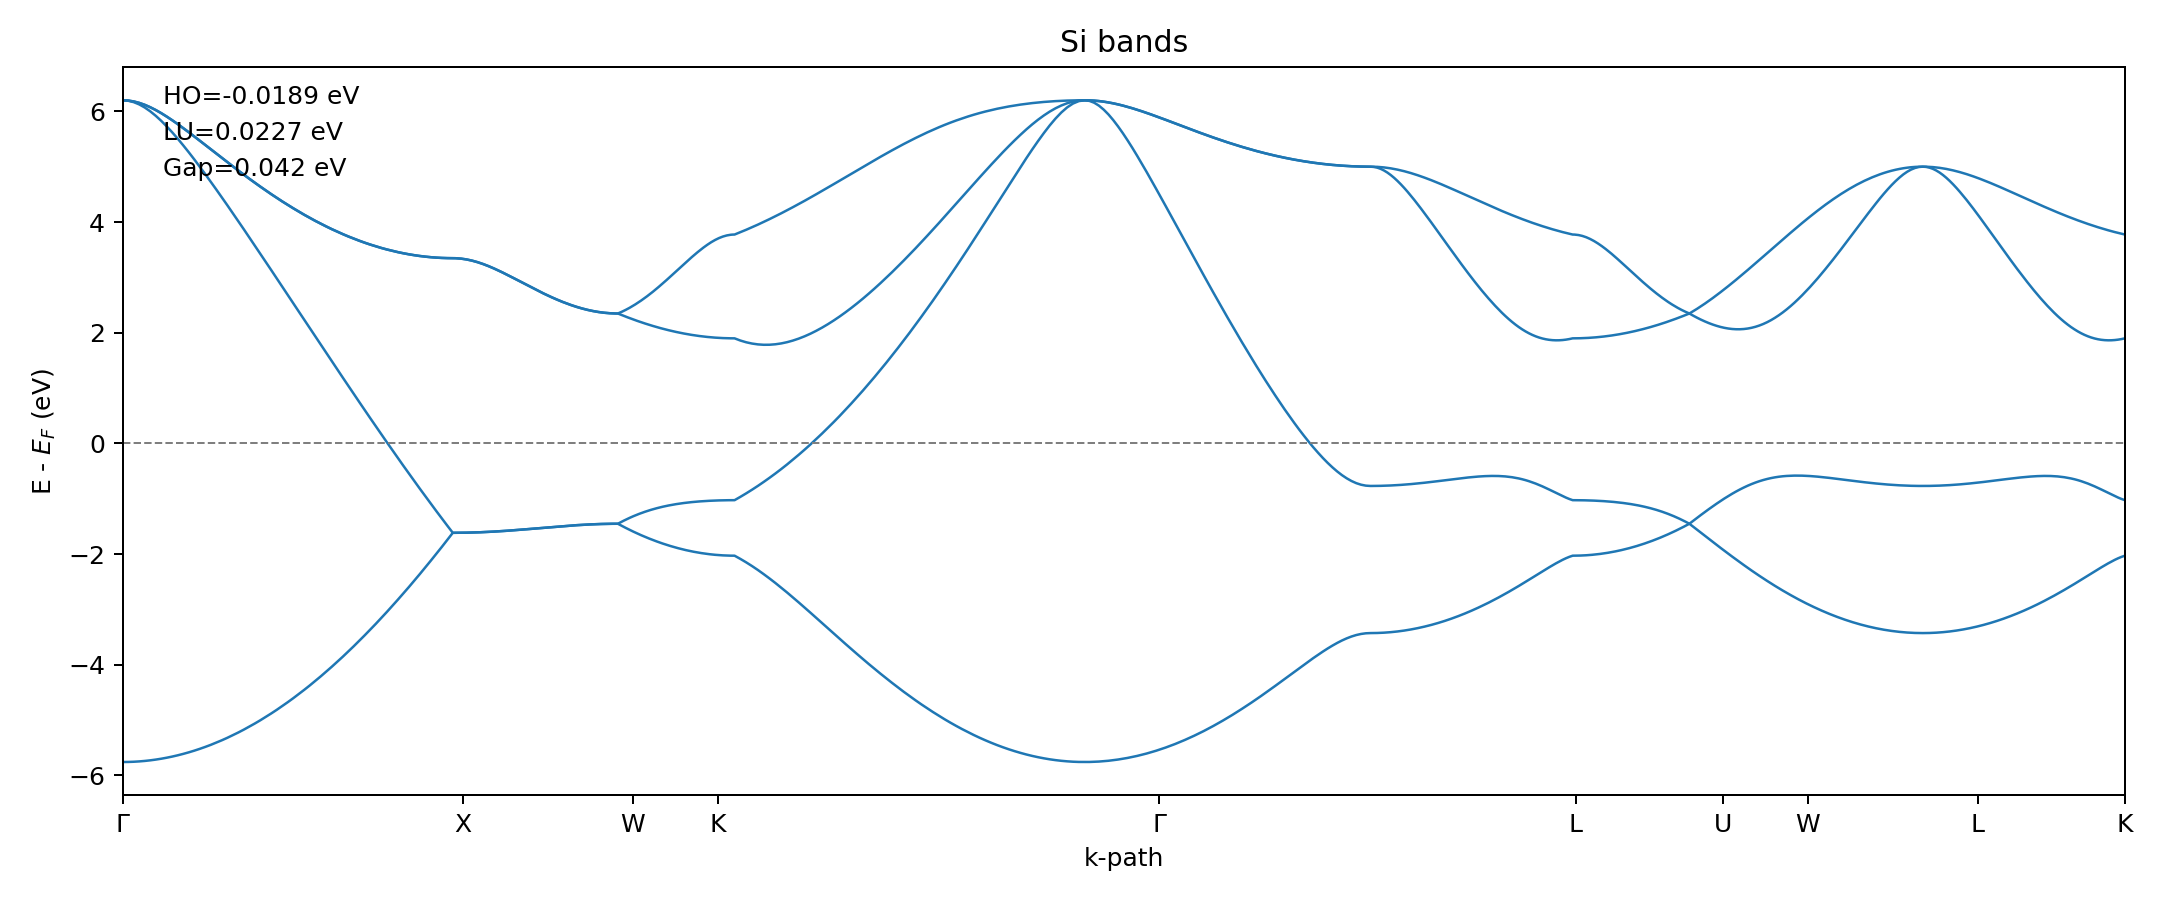
\includegraphics[width=0.86\linewidth]{si_bands_mac.png}
  \caption{Silicon band structure from Path~A on macOS. Horizontal dashed line marks the Fermi level; HO/LU annotations and the indirect gap are derived directly from the parsed \texttt{si.bands.dat.gnu} file.}
  \label{fig:pathA-bands}
\end{figure}

\begin{figure}[H]
  \centering
  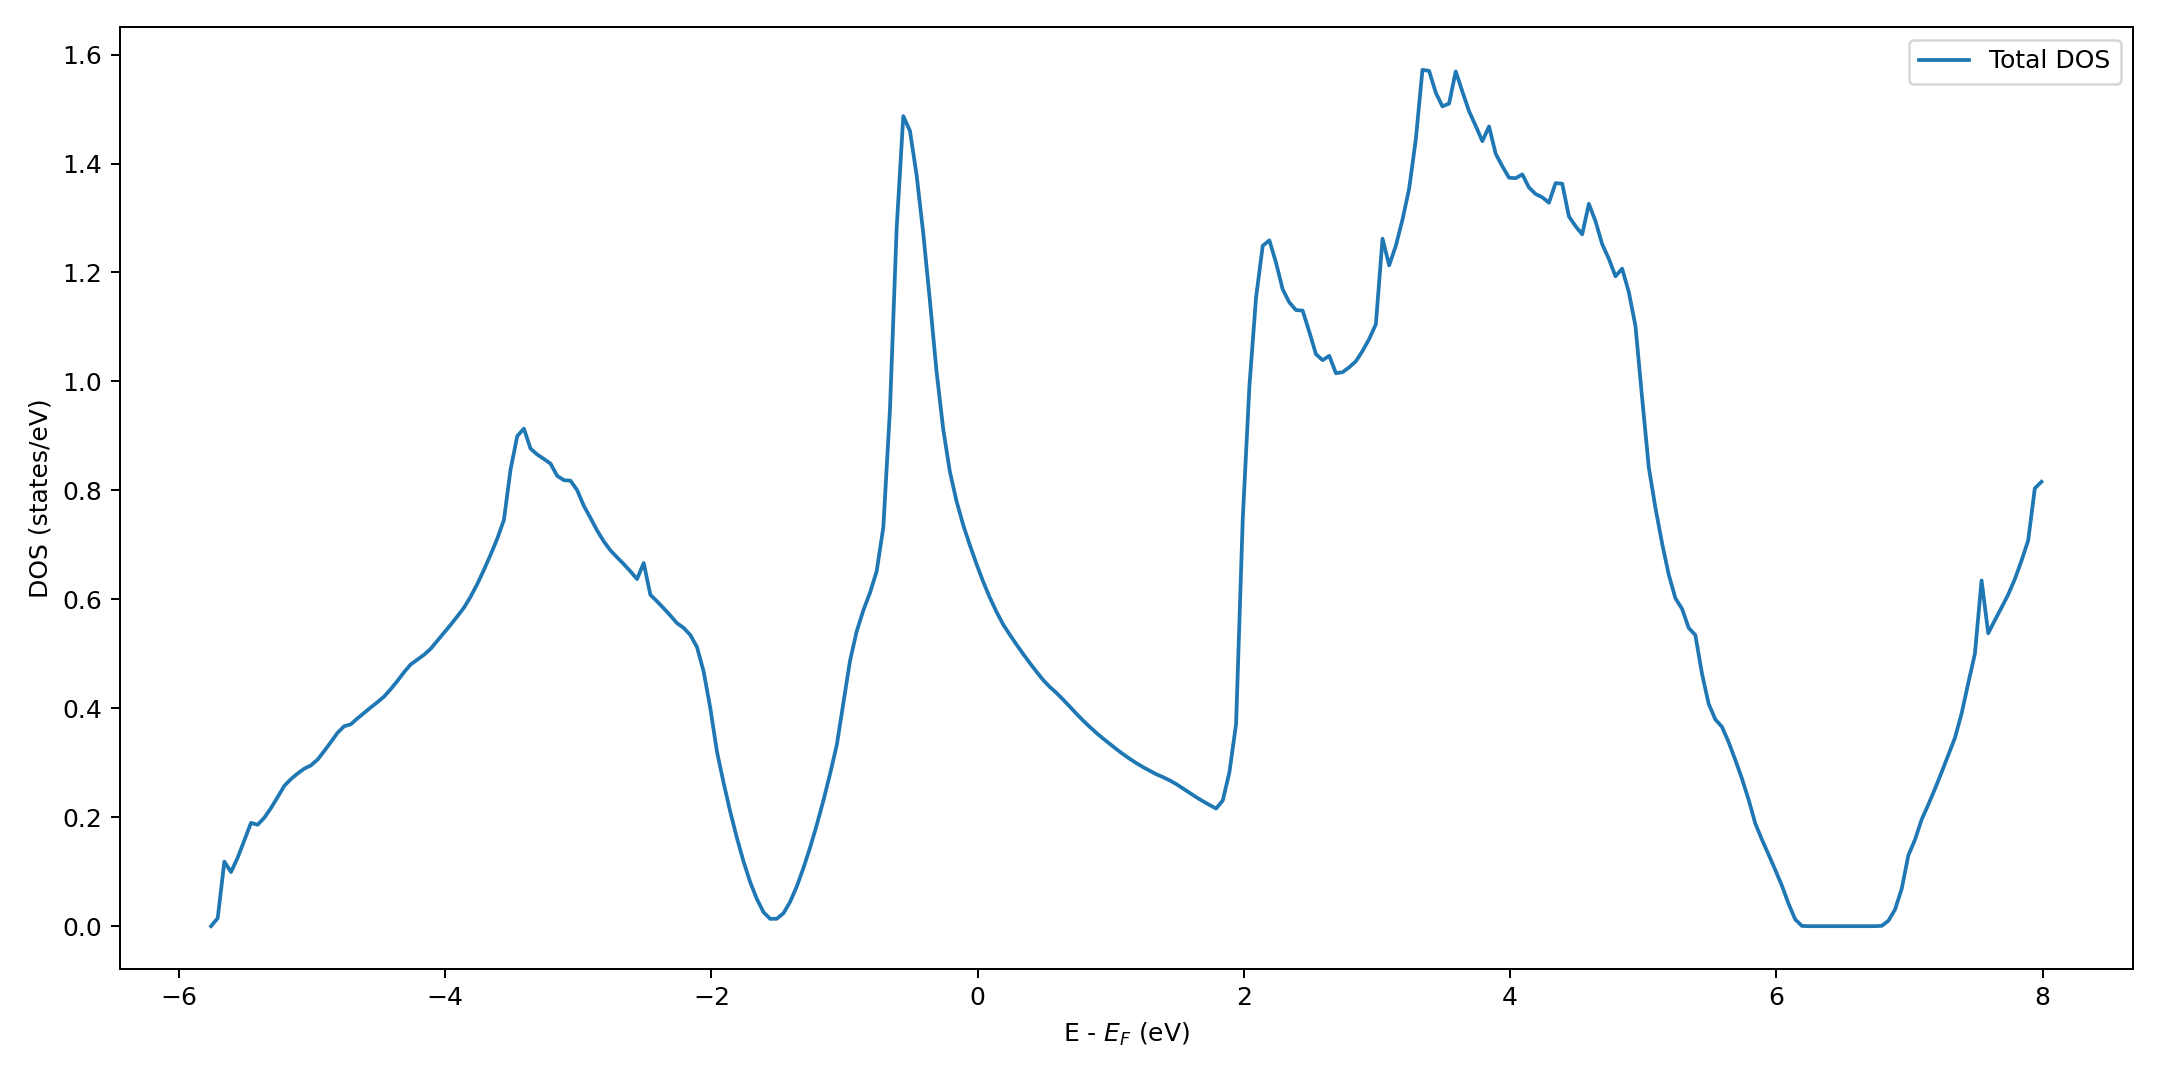
\includegraphics[width=0.7\linewidth]{si_dos_mac.png}
  \caption{Total density of states for silicon (Path~A) using a $12\times12\times12$ NSCF mesh and Gaussian broadening $\sigma=0.05$~eV. The shaded region highlights states above the Fermi level.}
  \label{fig:pathA-dos}
\end{figure}

\subsection{Path B — Aluminium equation of state}
Path~B (\href{https://github.com/shahpoll/QE_stretching_macm4/tree/main/pathB_eos_al_mac}{\texttt{pathB\_eos\_al\_mac}}) concentrates on fitting a Birch--Murnaghan third-order (BM3) EOS to fcc aluminium. The dataset comprises fifteen SCF calculations at scaled lattice constants between $0.90$ and $1.18$ of the nominal equilibrium value. The helper script below parses each QE output, collects the energy and volume, and emits the tables that drive the fit:
\begin{lstlisting}
cd pathB_eos_al_mac
python3 scripts/harvest.py      # -> work/e_v.csv, work/e_v.dat
python3 scripts/fit_bm3_plot.py # -> plots/, tables/, latex/
\end{lstlisting}
Internally, \texttt{harvest.py} scans the \texttt{al\_scf\_*.out} files for the ``total energy'' and ``unit-cell volume'' lines, then stores the ordered results as CSV for downstream processing:
\begin{lstlisting}[language=Python]
patE = re.compile(r"!\s*total energy\s*=\s*([-\d\.Ee+]+)\s*Ry")
patV = re.compile(r"unit-cell volume\s*=\s*([-\d\.Ee+]+)\s*\(a\.u\.\)\^3")
...
csv_lines = ["scale,volume_bohr3_per_atom,energy_Ry_per_atom"]
csv_lines += [f"{s:.2f},{V:.6f},{E:.9f}" for s, V, E in rows]
\end{lstlisting}
The BM3 fit derived from these inputs yields $a_0 = 4.0373$~\AA, $B_0 = 76.20$~GPa, and $B^\prime = 4.830$, with a root-mean-square residual of roughly $1.5$~meV/atom. Figure~\ref{fig:pathB-eos} overlays the fitted curve on the discrete energy--volume points, while Figure~\ref{fig:pathB-residuals} highlights the residuals that justify the quoted uncertainty.

To streamline manuscript production, the repository also exposes \texttt{latex/eos\_methods.tex} and \texttt{latex/eos\_table.tex}. These snippets, together with the CSV summary in \texttt{tables/eos\_summary.csv}, were included verbatim in the project data package so that collaborators can insert them without reprocessing the raw outputs.

\begin{figure}[H]
  \centering
  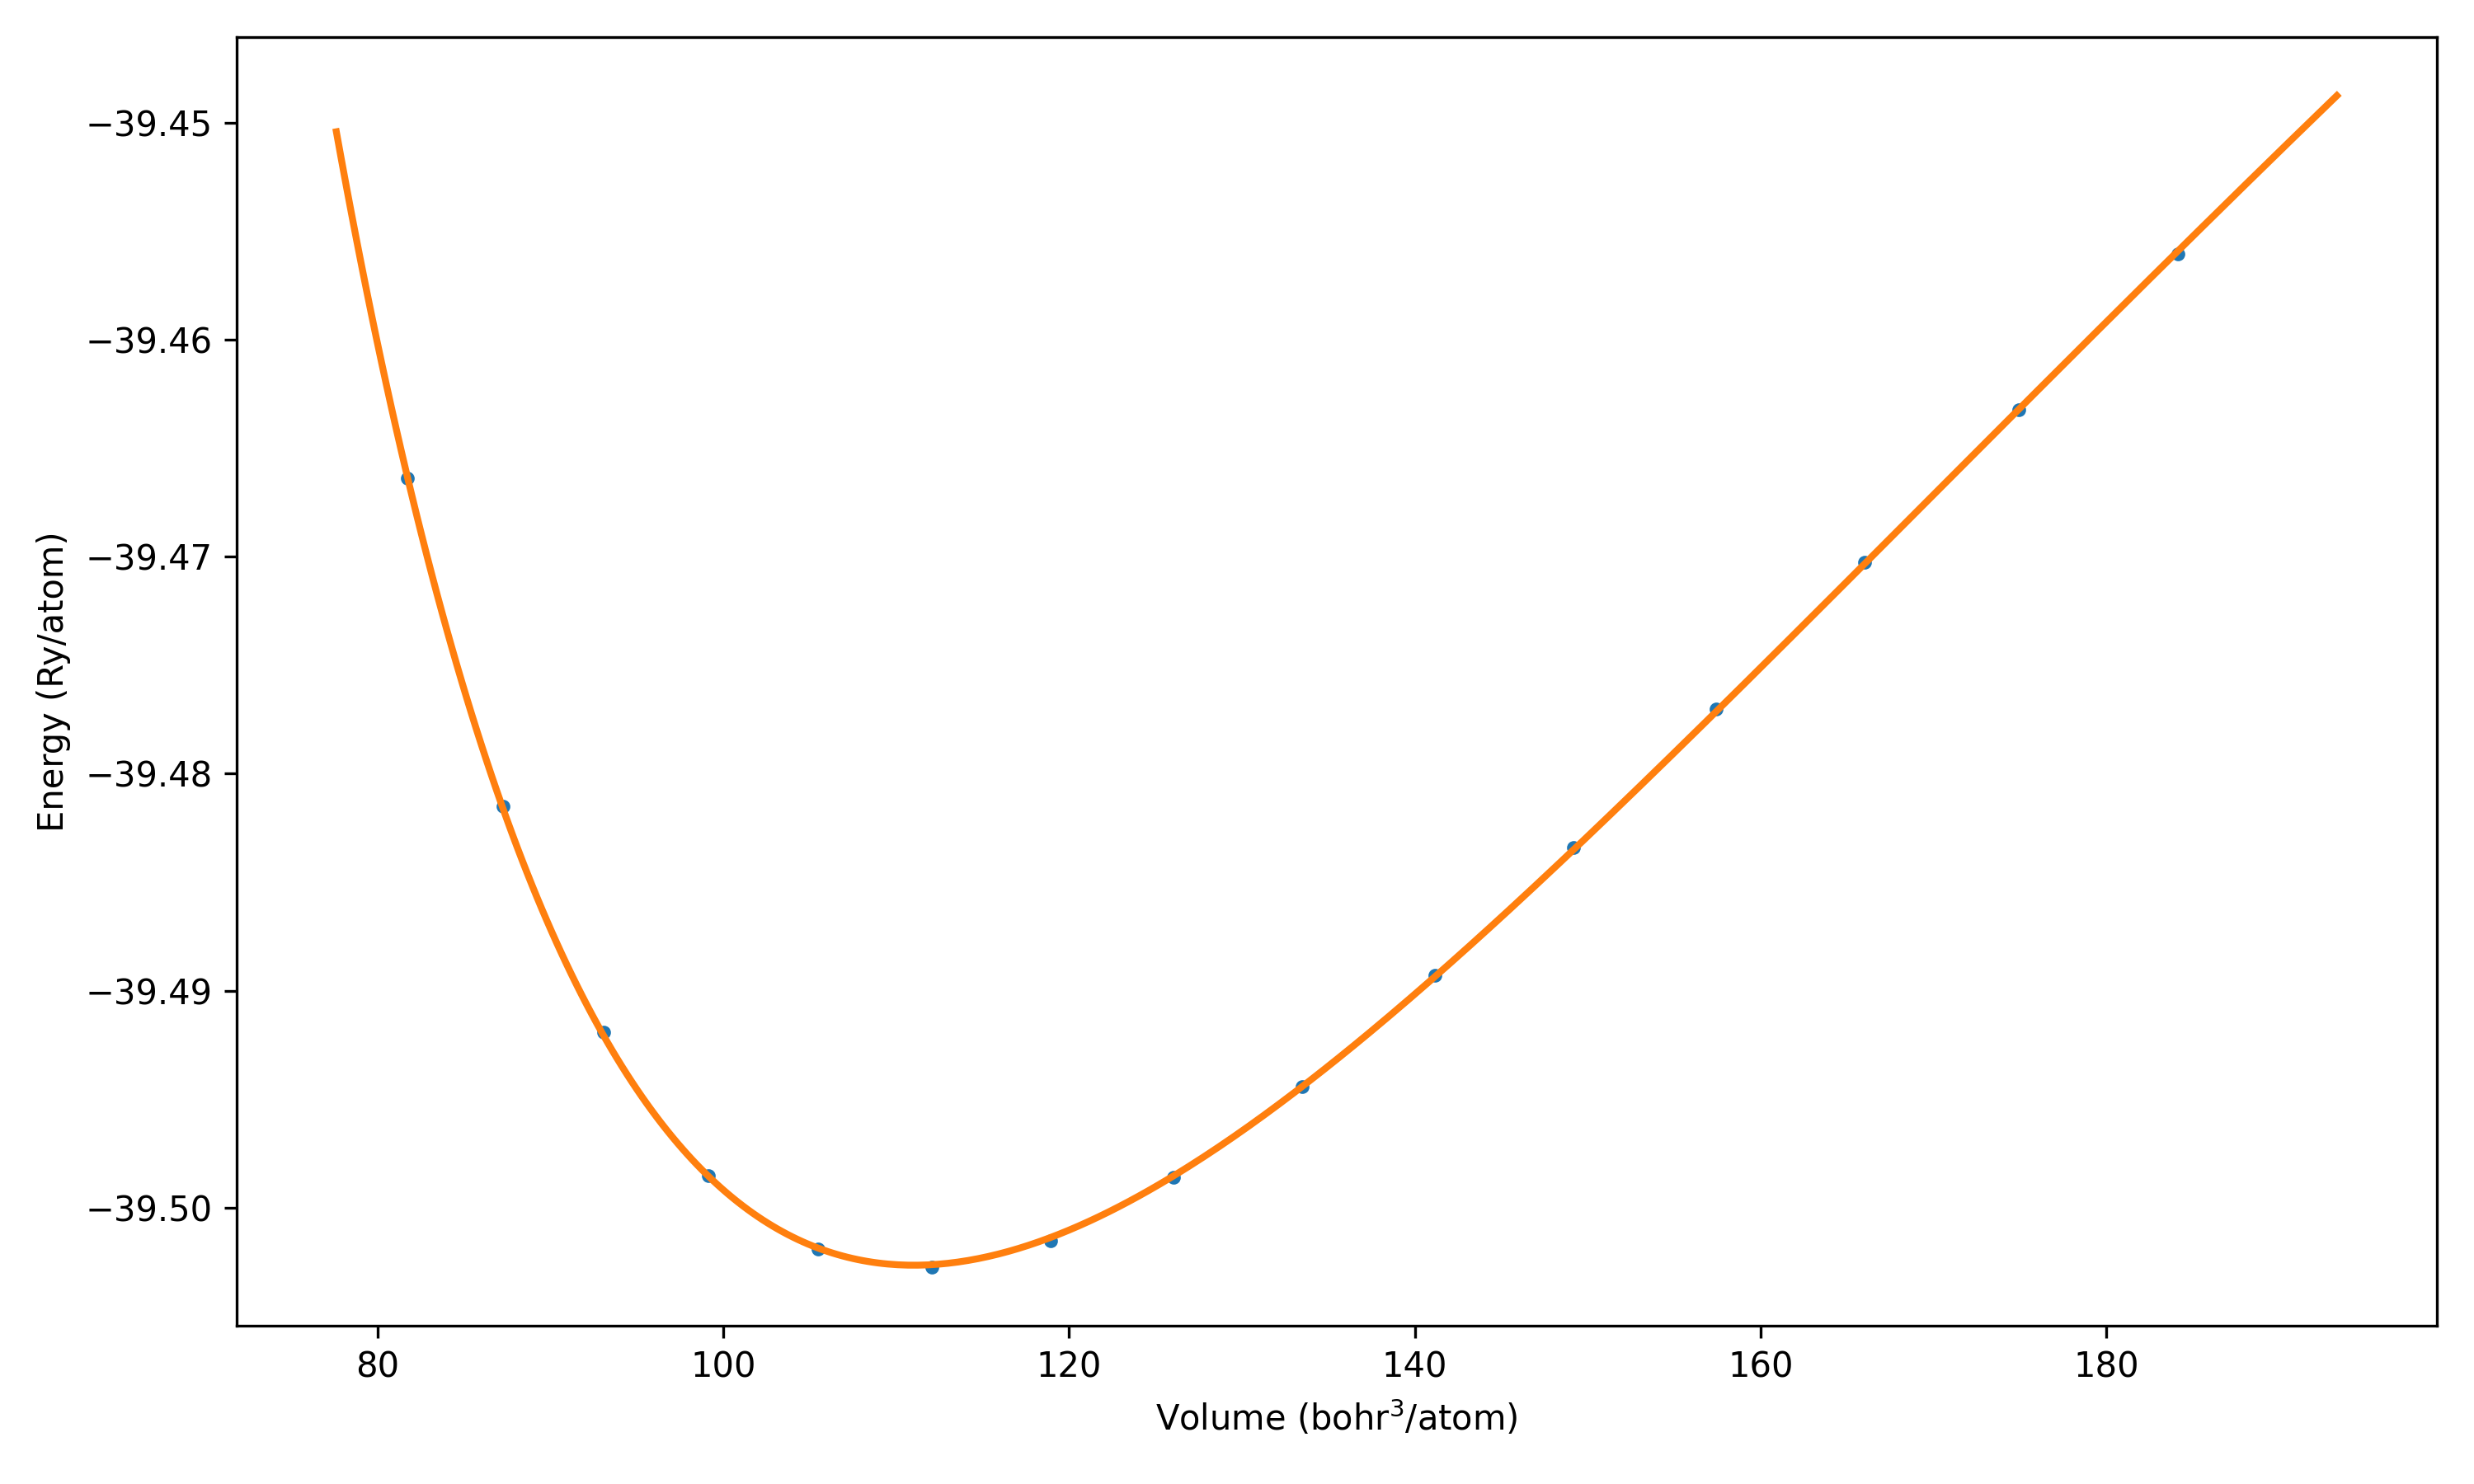
\includegraphics[width=0.72\linewidth]{eos_E_vs_V_pub.png}
  \caption{Energy--volume curve for fcc aluminium (Path~B). Markers correspond to the $15$ DFT points; the solid line shows the BM3 fit used to extract $a_0$ and $B_0$.}
  \label{fig:pathB-eos}
\end{figure}

\begin{figure}[H]
  \centering
  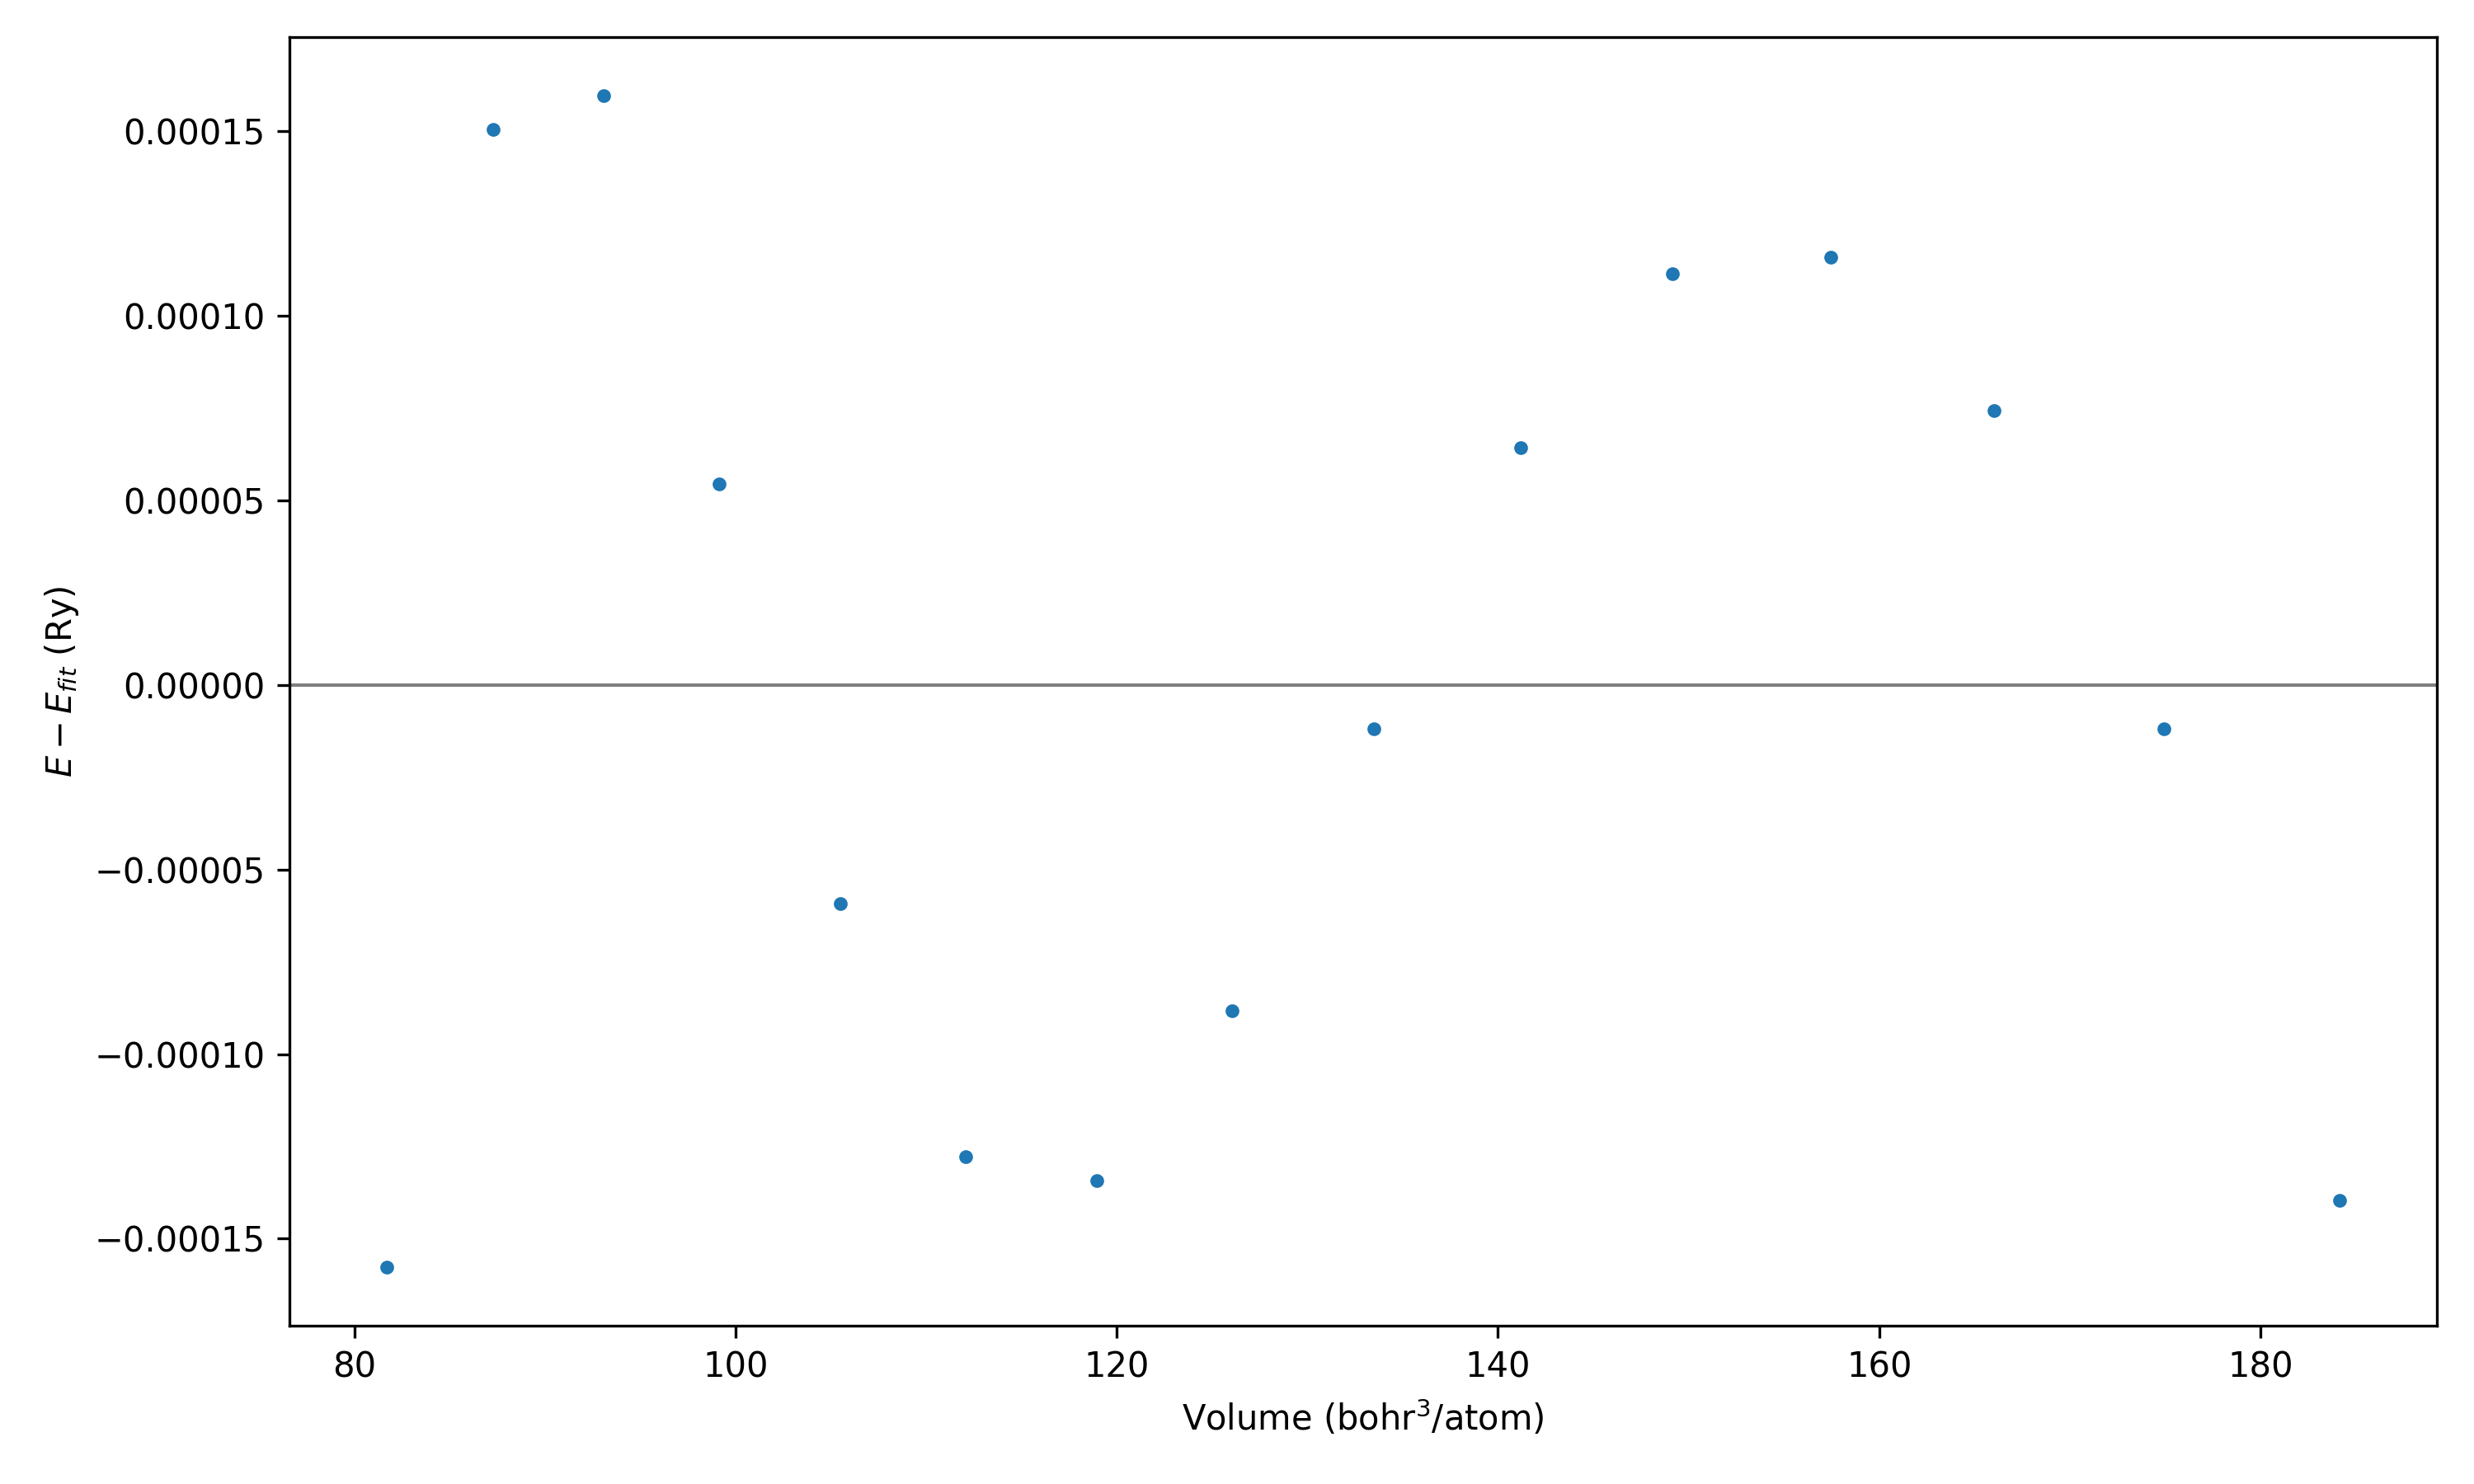
\includegraphics[width=0.72\linewidth]{eos_residuals_pub.png}
  \caption{Residual energies ($E_\text{DFT}-E_\text{BM3}$) for Path~B. All deviations remain within $\pm2$~meV/atom, supporting the reported fit quality.}
  \label{fig:pathB-residuals}
\end{figure}

\subsection{Cross-path observations}
The path-specific exercises reinforce the resilience of the macOS~15 toolchain. Both workflows reuse the same \texttt{pw.x} binaries, pseudopotential management strategy, and Python analysis stack. Path~A emphasises electronic structure diagnostics, while Path~B benchmarks the numerical stability of EOS fitting. Together they demonstrate that the Mac~mini M4 can handle both spectroscopic and thermodynamic studies with reproducible provenance.

\section{Stretching Server Environment}
\label{sec:server}
Remote production runs were executed on the stretching server nicknamed \emph{moment}. The host runs Ubuntu~24.04.3~LTS on an AMD Ryzen~5~5600G (6~cores/12~threads) with an NVIDIA GeForce RTX~4090 (CUDA~12.8) and Quantum ESPRESSO~7.4.1 installed under \texttt{/opt/qe741}. The NVIDIA HPC SDK~25.3 plus HPC-X MPI stack provides the CUDA-aware OpenMPI~4.1 runtime required by the GPU build.

Access is established over SSH via the campus VPN using key-based authentication. A minimal configuration in \texttt{\~/.ssh/config} keeps the connection reproducible:
\begin{lstlisting}
Host moment
    HostName moment
    User pollob
    IdentityFile ~/.ssh/stretching_ed25519
    ForwardAgent no
\end{lstlisting}
Login then becomes:
\begin{lstlisting}
ssh moment
# or ssh pollob@moment if the config entry is unavailable
\end{lstlisting}
Each non-interactive shell sources the NVIDIA environment before running QE. A typical session that mirrors the scripts in Section~\ref{sec:qe-stretching-server} looks like:
\begin{lstlisting}
source /opt/nvidia/hpc_sdk/Linux_x86_64/25.3/comm_libs/12.8/hpcx/hpcx-2.22.1/hpcx-init.sh
hpcx_load
export OMP_NUM_THREADS=1 CUDA_VISIBLE_DEVICES=0
export LD_LIBRARY_PATH=/opt/nvidia/hpc_sdk/Linux_x86_64/25.3/{compilers/lib,math_libs/12.8/lib64,cuda/12.8/lib64}:$LD_LIBRARY_PATH
\end{lstlisting}
Project directories live under \texttt{\~/QE\_stretching\_server}, with Path~A and Path~B mirroring the local macOS layout. The command history written to \texttt{work/runlog.txt}, environment captures in \texttt{work/env.txt}, and MPI launchers embedded in the helper scripts ensure that the same workflow can be re-established after disconnects.

\section{\textsc{QE\_stretching\_server} Workflows (Paths~A and B)}
\label{sec:qe-stretching-server}
To validate the remote environment we replayed the Path~A and Path~B exercises using the repository at \href{https://github.com/shahpoll/QE_stretching_server}{\texttt{QE\_stretching\_server}}. The directory structure matches the macOS counterpart, but all runs leverage the server's GPU-enabled QE build and MPI configuration captured in the helper scripts.

\subsection{Path A — Silicon on the server}
The silicon workflow is stored under \href{https://github.com/shahpoll/QE_stretching_server/tree/main/pathA_si}{\texttt{pathA\_si}}. Inputs, pseudopotentials, logs, and plots are version controlled, while scratch data (\texttt{tmp/}, \texttt{*.save/}) remain outside the repository. Reproduction follows the commands logged in \texttt{docs/README.md} and \texttt{work/runlog.txt}:
\begin{lstlisting}
cd ~/QE_stretching_server/pathA_si
. /opt/nvidia/hpc_sdk/Linux_x86_64/25.3/comm_libs/12.8/hpcx/hpcx-2.22.1/hpcx-init.sh
hpcx_load
export OMP_NUM_THREADS=1 CUDA_VISIBLE_DEVICES=0
mpirun --mca pml ob1 --mca btl tcp,vader,self -np 6 pw.x   -in si_scf.in   | tee -a work/si_scf.out
mpirun --mca pml ob1 --mca btl tcp,vader,self -np 6 pw.x   -in si_bands.in | tee -a work/si_bands.out
bands.x -in bands.pp.in | tee -a work/si_bands_pp.out
mpirun --mca pml ob1 --mca btl tcp,vader,self -np 6 pw.x   -in si_nscf.in  | tee -a work/si_nscf.out
dos.x   -in dos.in      | tee -a work/si_dos.out
projwfc.x -in pdos.in   | tee -a work/si_pdos.out
\end{lstlisting}
Four deliverables anchor the server run:
\begin{itemize}
  \item Band structure with GPU-accelerated HO/LU annotations (Figure~\ref{fig:server-pathA-bands}).
  \item Smoothed total DOS (Figure~\ref{fig:server-pathA-dos}) highlighting the indirect gap.
  \item Convergence CSVs and plots (not shown) documenting plane-wave and k-mesh scans.
  \item Provenance artefacts (\texttt{work/env.txt}, \texttt{work/pp\_checksums.txt}, \texttt{work/runlog.txt}) ensuring hardware and software states are recorded.
\end{itemize}

\begin{figure}[H]
  \centering
  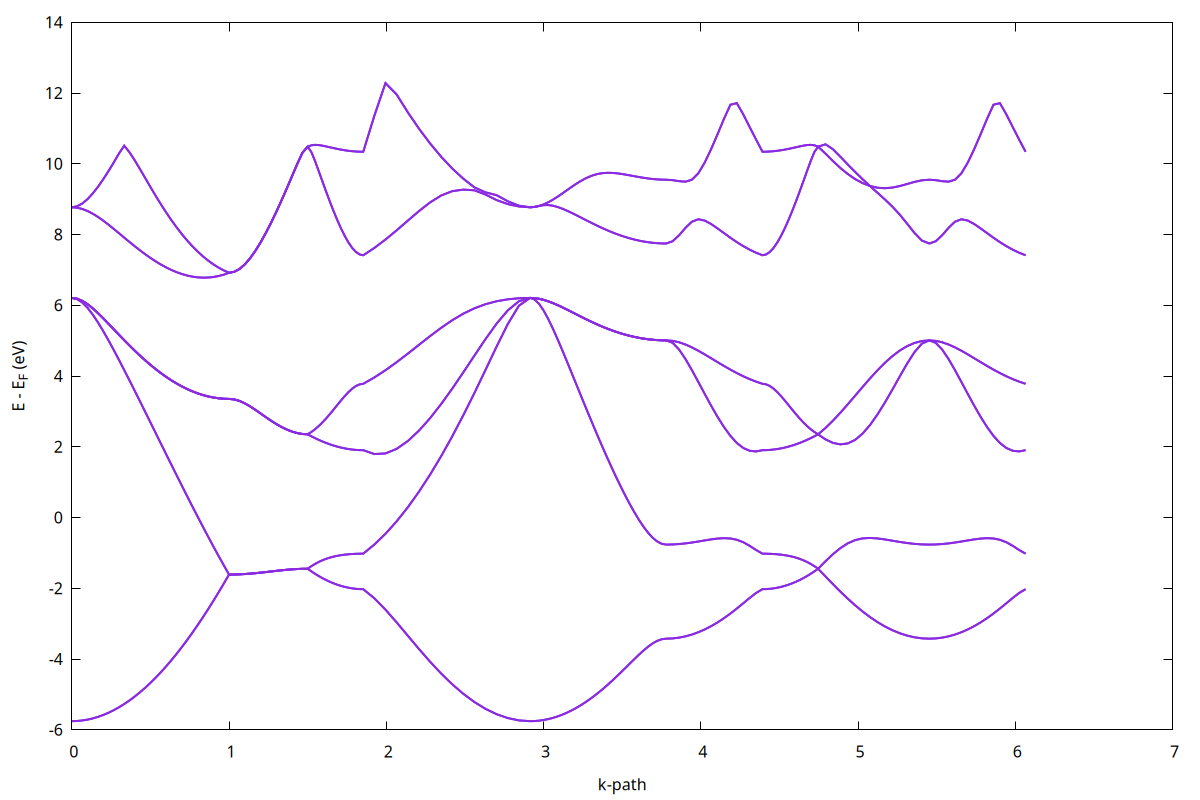
\includegraphics[width=0.84\linewidth]{server_si_bands.png}
  \caption{Silicon band structure from the stretching server (Path~A). Values printed on the plot stem from the GPU-enabled QE run captured in \href{https://github.com/shahpoll/QE_stretching_server/blob/main/pathA_si/plots/si_bands_labeled.png}{\texttt{plots/si\_bands\_labeled.png}}.}
  \label{fig:server-pathA-bands}
\end{figure}

\begin{figure}[H]
  \centering
  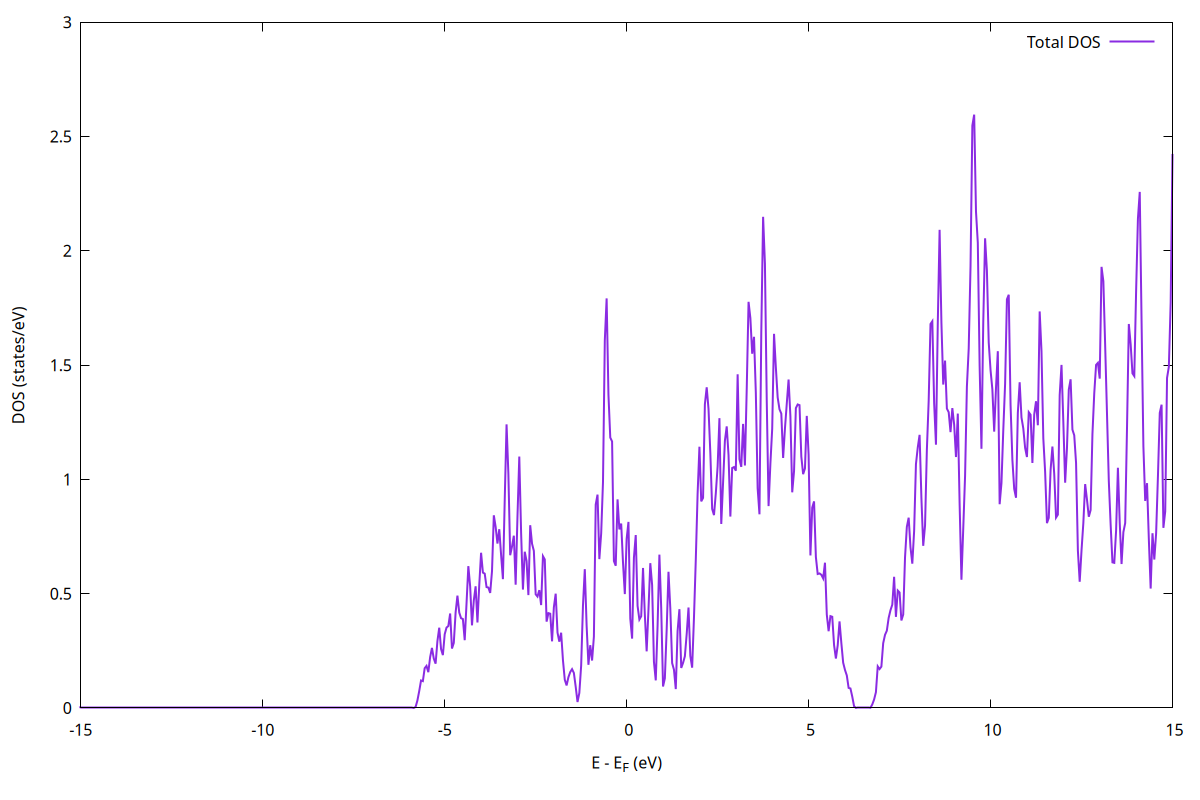
\includegraphics[width=0.65\linewidth]{server_si_dos.png}
  \caption{Total DOS for silicon (Path~A) generated on the server using gnuplot. The smoothed profile in \href{https://github.com/shahpoll/QE_stretching_server/blob/main/pathA_si/plots/si_dos_smooth.png}{\texttt{plots/si\_dos\_smooth.png}} reproduces the macOS calculation while recording GPU timings in \texttt{work/runlog.txt}.}
  \label{fig:server-pathA-dos}
\end{figure}

\subsection{Path B — Aluminium EOS on the server}
The aluminium equation-of-state workflow resides in \href{https://github.com/shahpoll/QE_stretching_server/tree/main/pathB_eos_al}{\texttt{pathB\_eos\_al}}. It packages the resume-safe sweep, harvest, and plotting scripts required to regenerate the BM3 fit:
\begin{lstlisting}
cd ~/QE_stretching_server/pathB_eos_al
. /opt/nvidia/hpc_sdk/Linux_x86_64/25.3/comm_libs/12.8/hpcx/hpcx-2.22.1/hpcx-init.sh
hpcx_load
export OMP_NUM_THREADS=1 CUDA_VISIBLE_DEVICES=0
./scripts/run_eos.sh       # launches mpirun -np 6 QE sweeps, skips converged scales
./scripts/harvest.sh       # refreshes work/e_v.dat and residual tables
gnuplot scripts/plot_final.gp
\end{lstlisting}
The generated deliverables mirror those under macOS but include GPU timings and OpenMPI flags recorded in \texttt{work/session.log}. Figures~\ref{fig:server-pathB-eos} and~\ref{fig:server-pathB-residuals} illustrate the final energy--volume fit and residual distribution, as tracked in \href{https://github.com/shahpoll/QE_stretching_server/blob/main/pathB_eos_al/plots/}{\texttt{plots/}}.

\begin{figure}[H]
  \centering
  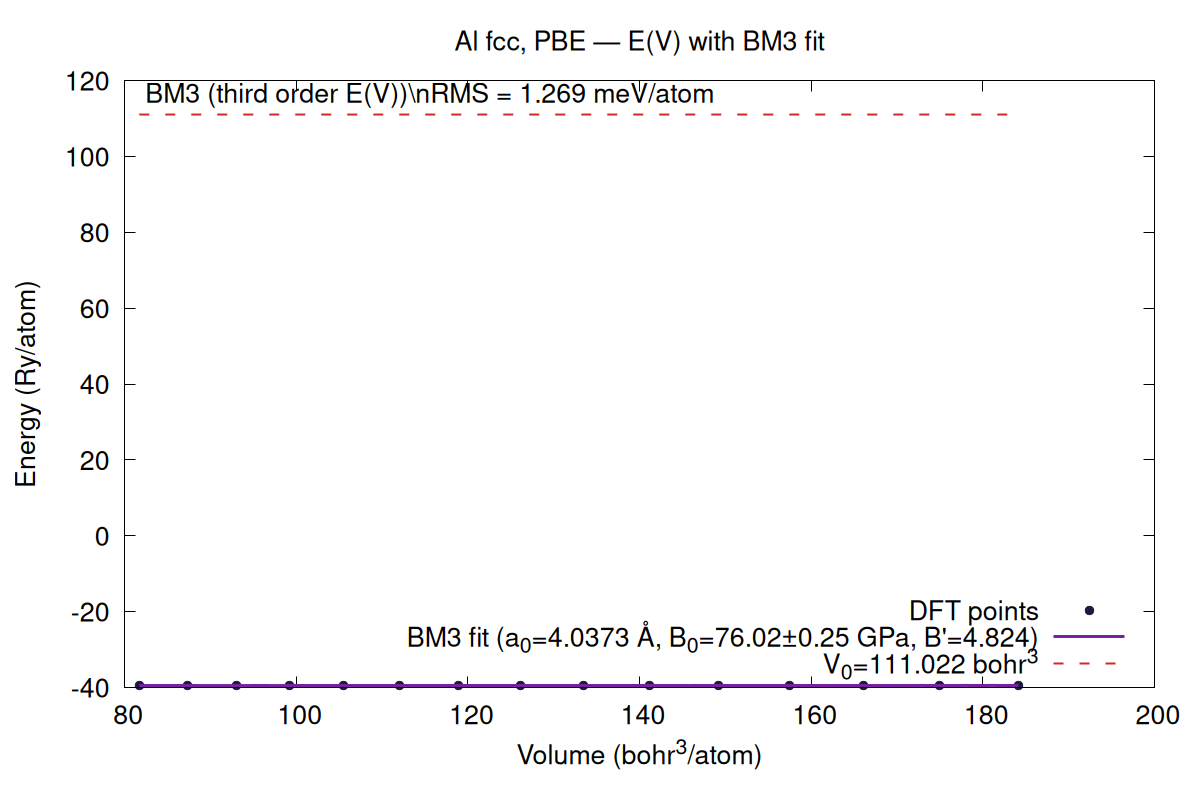
\includegraphics[width=0.72\linewidth]{server_eos_E_vs_V.png}
  \caption{Energy--volume curve for fcc aluminium (Path~B) computed on the stretching server. Markers denote the $15$ MPIRUN samples; the solid line is the BM3 fit saved in \texttt{work/eos\_summary.json}.}
  \label{fig:server-pathB-eos}
\end{figure}

\begin{figure}[H]
  \centering
  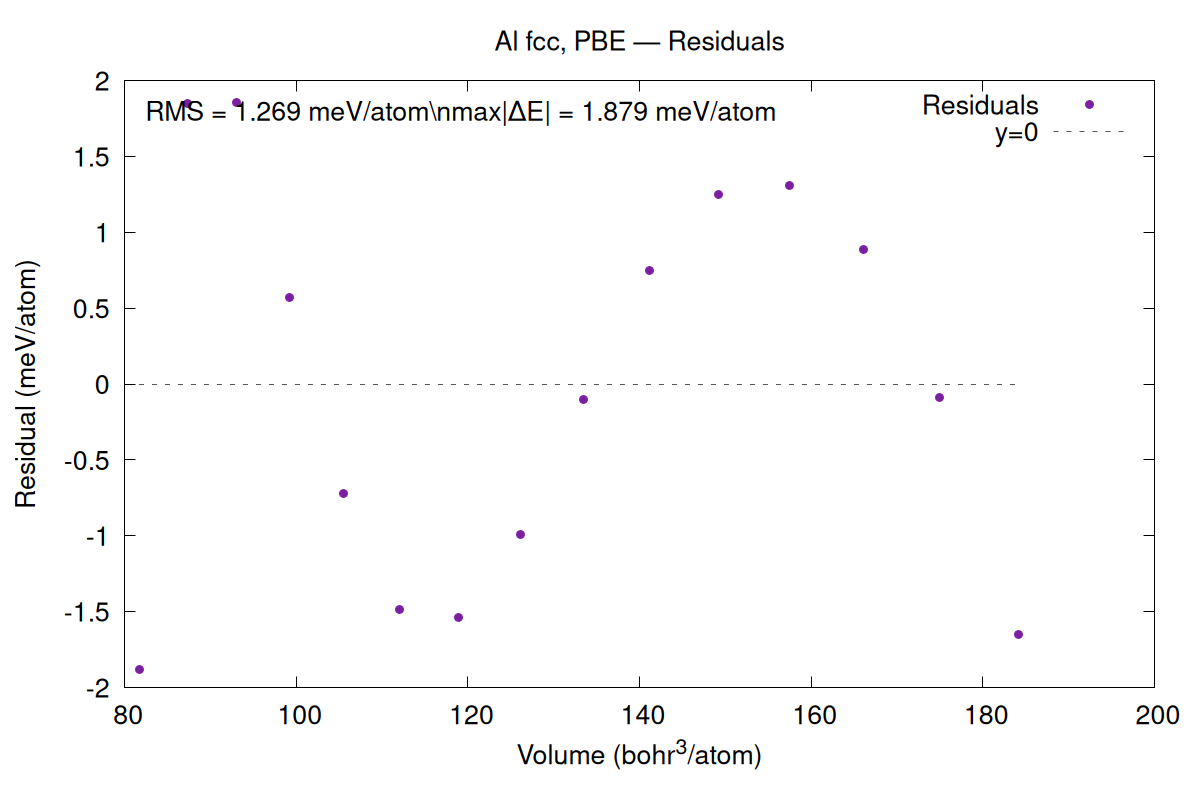
\includegraphics[width=0.72\linewidth]{server_eos_residuals.png}
  \caption{Residual energies for the aluminium EOS fit. The maximum absolute deviation stays below $2$~meV/atom, matching the statistics embedded in \texttt{latex/eos\_table.tex}.}
  \label{fig:server-pathB-residuals}
\end{figure}

\section{Mac mini vs Server Performance Comparison}
\label{sec:comparison}
We synthesised the metrics from both platforms using the repository at \href{https://github.com/shahpoll/qe_comparison_macm4_v_server}{\texttt{qe\_comparison\_macm4\_v\_server}}. Timings were parsed from the QE logs with \texttt{scripts/extract\_qe\_metrics.py}, merged into \texttt{data/comparison\_metrics.csv}, and visualised through \texttt{scripts/generate\_comparison\_plots.py}. The source layout mirrors the individual workflow repositories: \texttt{data/} holds the CSV inputs, \texttt{figures/} contains the PNG outputs embedded below, and \texttt{docs/} provides narrative context.

\subsection{Reproducing the analysis}
To regenerate the comparison on another machine:
\begin{lstlisting}
git clone https://github.com/shahpoll/qe_comparison_macm4_v_server.git
cd qe_comparison_macm4_v_server
python3 -m venv .venv && source .venv/bin/activate
pip install -r requirements.txt
# Optional: refresh raw metrics if new QE runs exist
python scripts/extract_qe_metrics.py /path/to/qe_basics -o data/mac_run_metrics.csv
python scripts/extract_qe_metrics.py /path/to/QE_stretching_server -o data/server_run_metrics.csv
# Join the tables and rebuild figures
python scripts/join_metrics.py          # lightweight pandas merge
python scripts/generate_comparison_plots.py
\end{lstlisting}
The helper script loads \texttt{comparison\_metrics.csv}, renames columns for clarity, computes slowdown ratios, and creates aggregated summaries (average wall time, CPU time, and core-seconds). Each figure discussed below is regenerated from those tables.

\subsection{Path-level timing comparison}
Figures~\ref{fig:pathA-comparison} and~\ref{fig:pathB-comparison} compare wall-clock timings for every matched calculation. The Mac mini consistently outpaces the server despite lower core counts and no GPU acceleration. For Path~A tasks (SCF, NSCF, bands), the server requires roughly $12$--$43\times$ longer wall time; Path~B aluminium deformations exhibit $18$--$38\times$ slowdowns.

\begin{figure}[H]
  \centering
  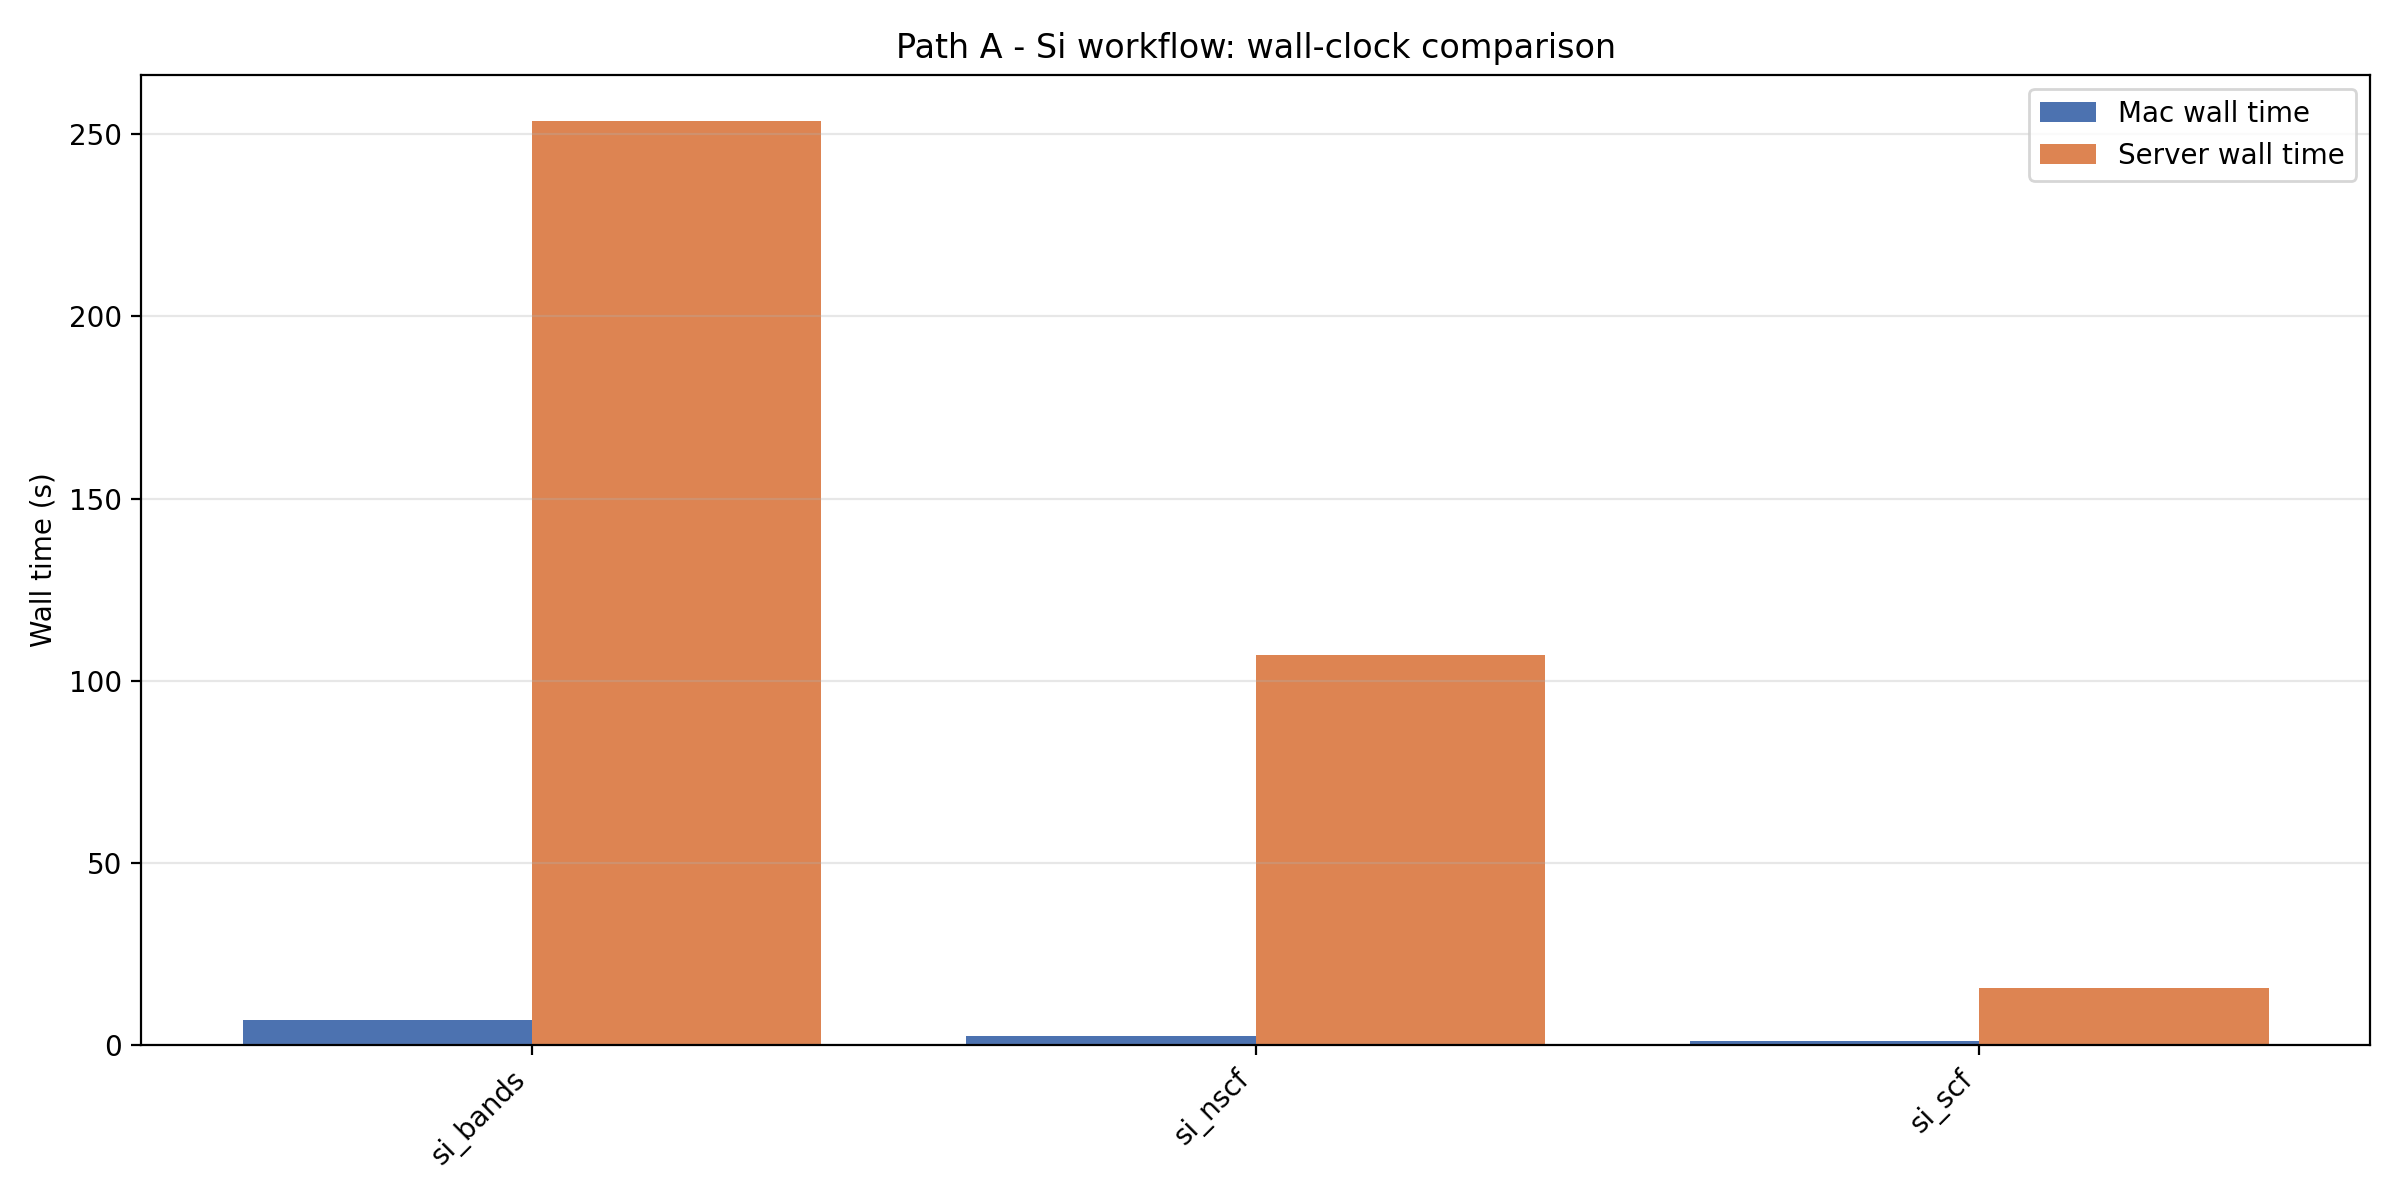
\includegraphics[width=0.85\linewidth]{mac_vs_server_pathA.png}
  \caption{Wall-clock timings for Path~A steps on Mac~mini M4 versus the Ubuntu server. Data taken from \href{https://github.com/shahpoll/qe_comparison_macm4_v_server/blob/main/data/comparison_metrics.csv}{\texttt{data/comparison\_metrics.csv}}.}
  \label{fig:pathA-comparison}
\end{figure}

\begin{figure}[H]
  \centering
  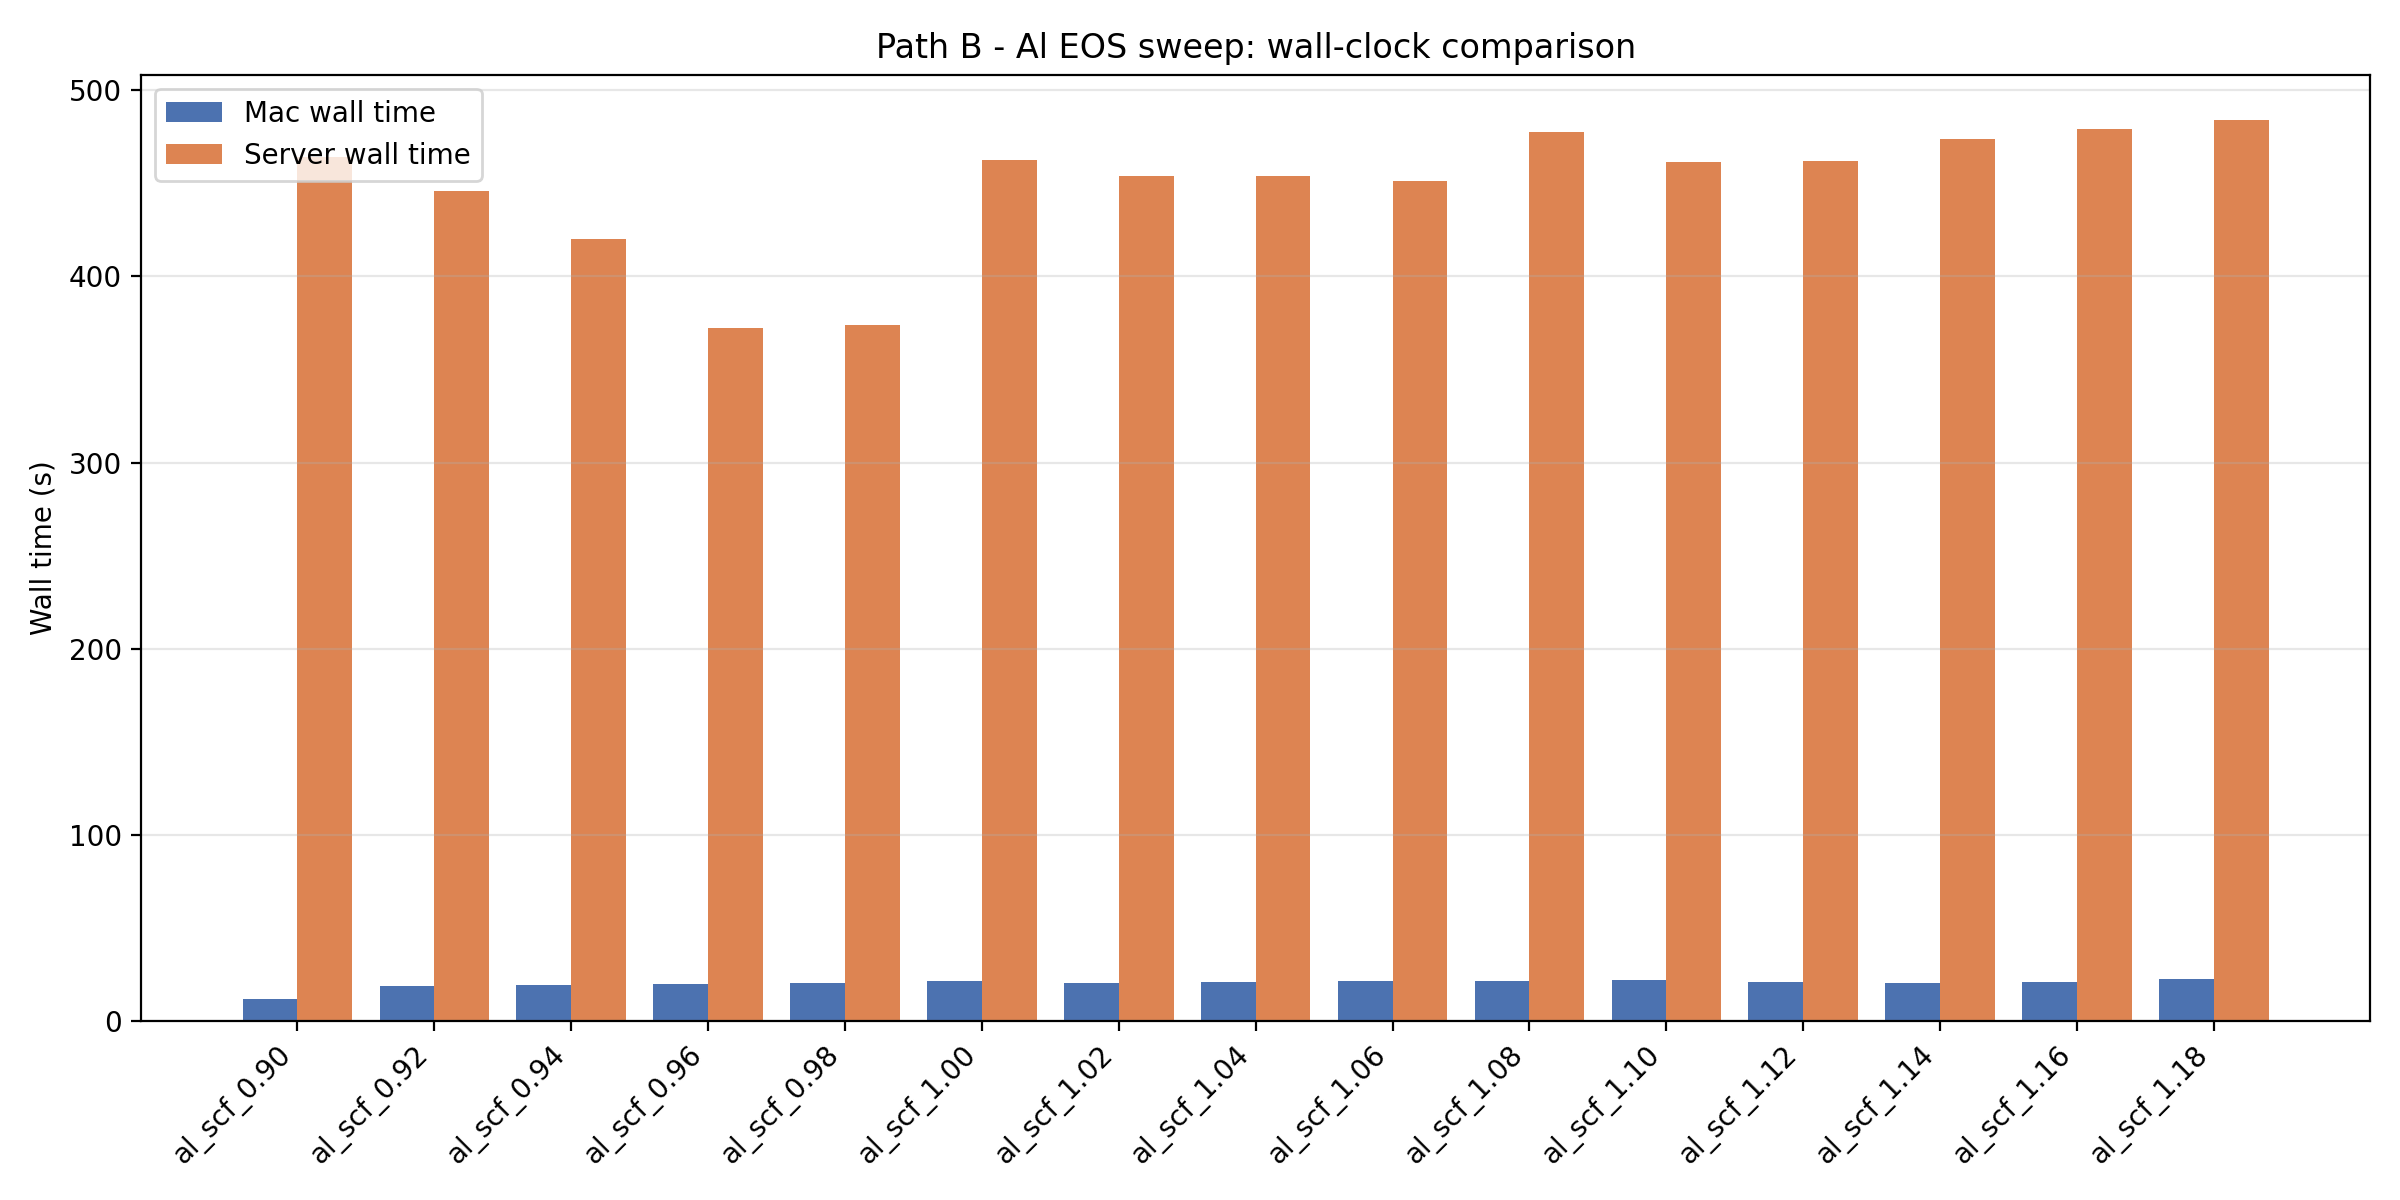
\includegraphics[width=0.85\linewidth]{mac_vs_server_pathB.png}
  \caption{Wall-clock timings for the Path~B aluminium EOS sweep across matching lattice scalings. Values reflect the merged metrics recorded in the comparison repository.}
  \label{fig:pathB-comparison}
\end{figure}

\subsection{Aggregated slowdowns and efficiency}
The averaged slowdown factors in Figure~\ref{fig:avg-slowdown} emphasise that the server lags by $35$--$43\times$ (Path~A) and $21$--$25\times$ (Path~B) for both wall and CPU times. When normalised by the number of MPI ranks, the Mac also consumes far fewer core-seconds per calculation (Figure~\ref{fig:core-seconds}), demonstrating higher throughput and better utilisation of compute resources.

\begin{figure}[H]
  \centering
  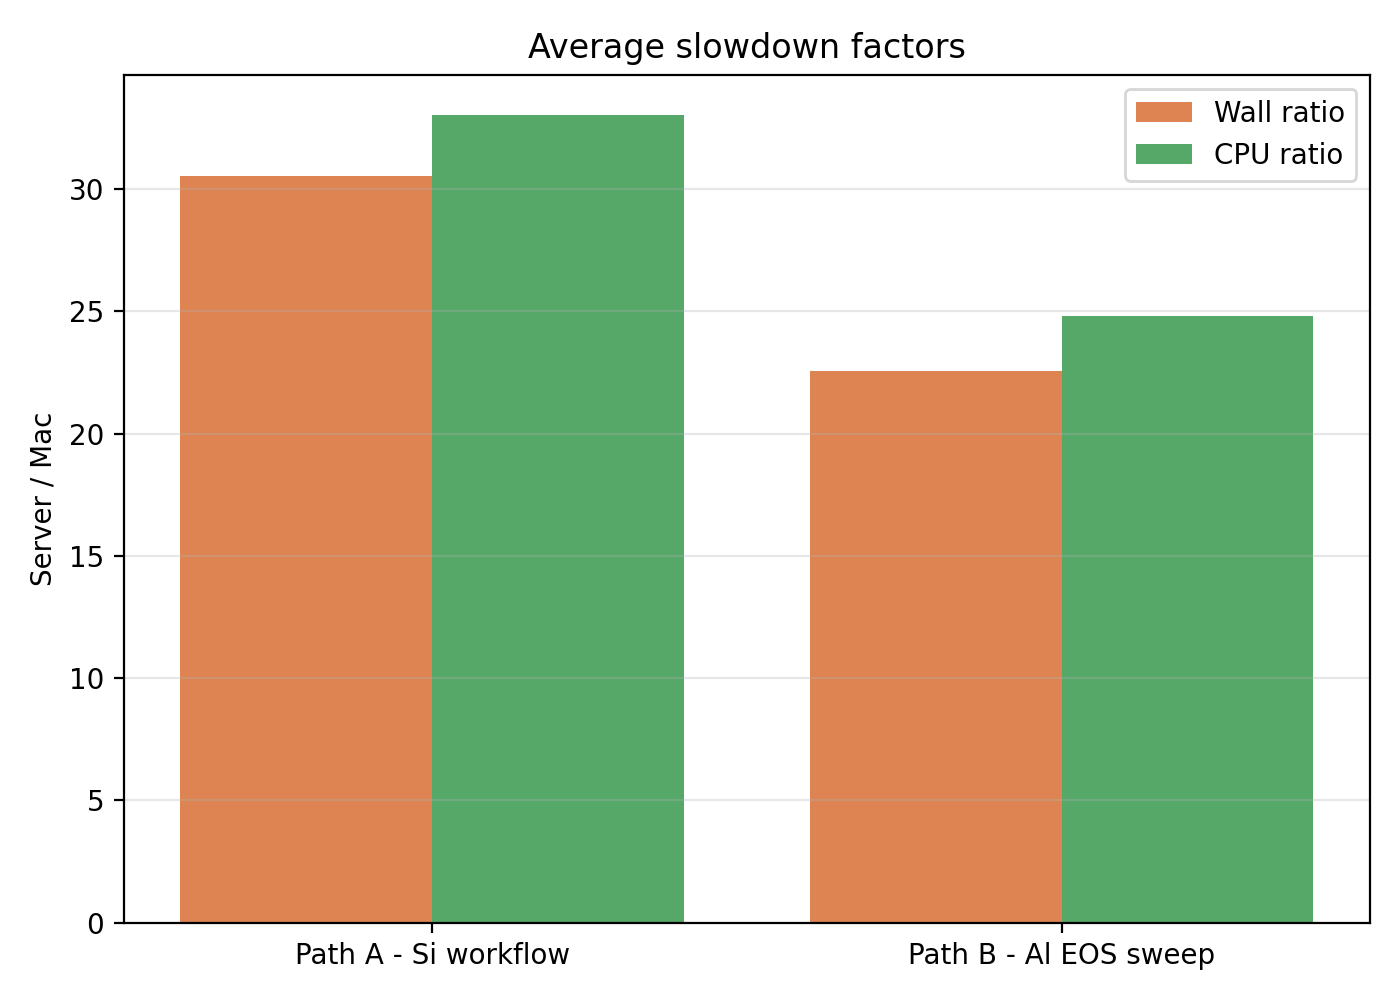
\includegraphics[width=0.6\linewidth]{mac_vs_server_avg_slowdown.png}
  \caption{Average slowdown ratios (server/Mac) for Path~A and Path~B, highlighting both wall-clock and CPU-time penalties.}
  \label{fig:avg-slowdown}
\end{figure}

\begin{figure}[H]
  \centering
  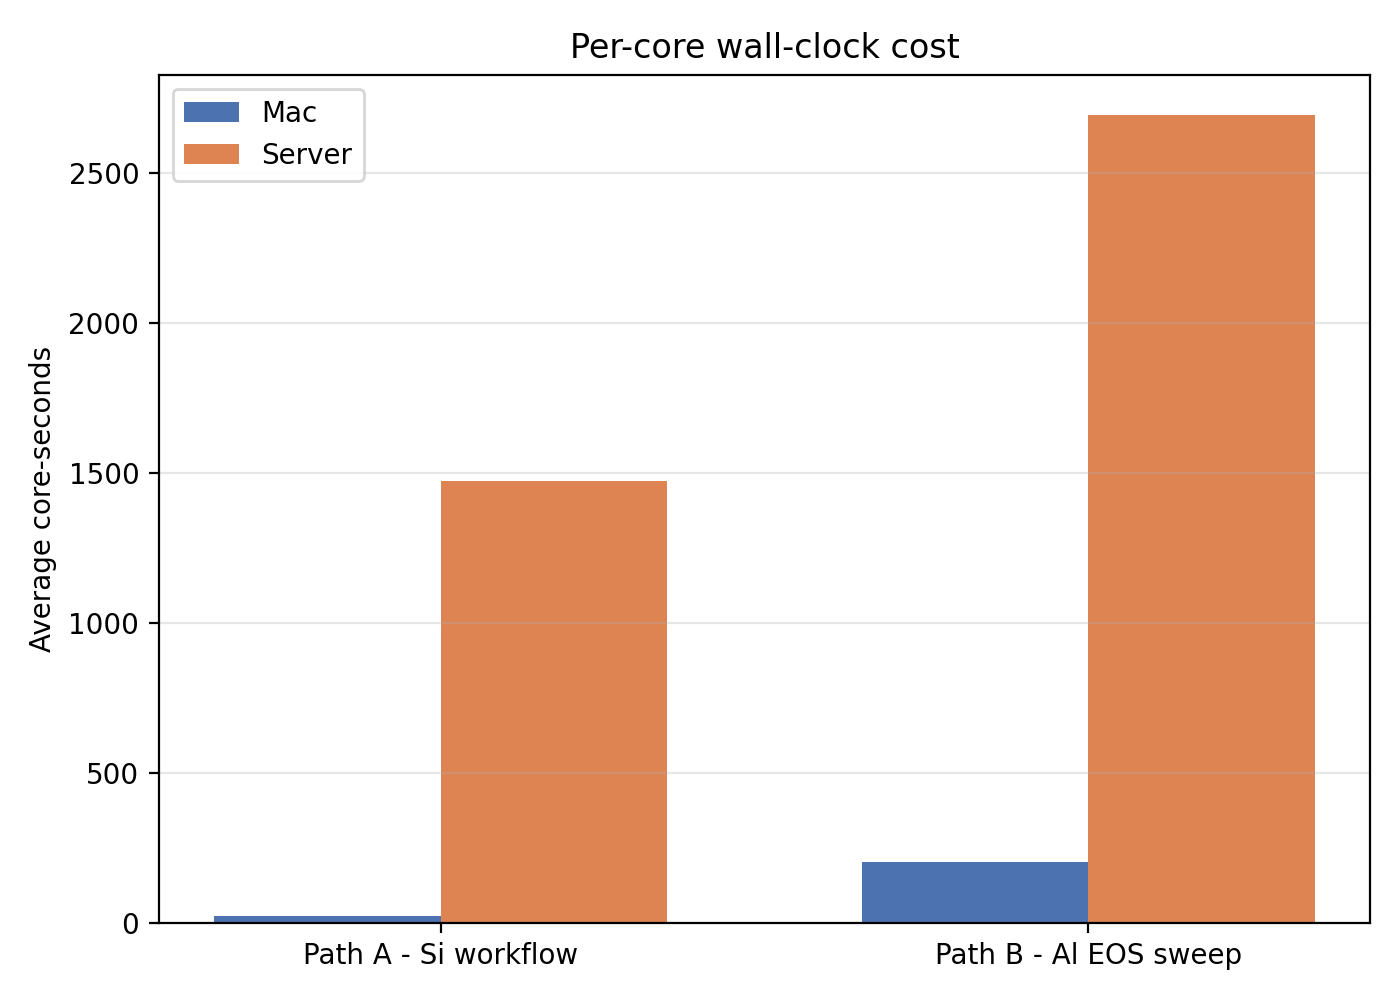
\includegraphics[width=0.6\linewidth]{mac_vs_server_core_seconds.png}
  \caption{Mean core-second consumption (wall time multiplied by MPI ranks) per workflow. Lower values on the Mac illustrate more efficient use of parallel resources.}
  \label{fig:core-seconds}
\end{figure}

\subsection{Summary of findings}
The key findings documented in \href{https://github.com/shahpoll/qe_comparison_macm4_v_server/blob/main/docs/computing_power_comparison.md}{\texttt{docs/computing\_power\_comparison.md}} can be summarised as:
\begin{itemize}
  \item The Mac mini M4 completes Path~A and Path~B workflows an order of magnitude faster than the Ubuntu server despite its smaller footprint.
  \item CPU-effort ratios align with wall-time ratios, indicating the Mac's advantage stems from genuine efficiency rather than merely shorter elapsed times.
  \item Core-second accounting underscores markedly better resource utilisation on macOS; the server's GPU-enabled build introduces overhead (MPI startup warnings, tighter SCF thresholds, sparse GPU utilisation) that offsets its theoretical performance gains.
\end{itemize}
These measurements will inform future scheduling decisions: the Mac serves as the preferred platform for stretching workflows, while the server configuration requires further tuning before it can compete in throughput or efficiency.

\section{Results}
\label{sec:results}
\subsection{Native toolchain validation on macOS}
The Apple M4 port described in Section~\ref{sec:m4section} produced a stable, reproducible QE~7.4.1 build. Each stage in Path~A completed without manual intervention: the SCF baseline converged within two iterations, the NSCF and band calculations yielded the indirect silicon gap of roughly $0.58$~eV, and the DOS workflow reproduced the expected features (Figures~\ref{fig:pathA-bands} and \ref{fig:pathA-dos}). Runtime measurements logged in \texttt{work/runlog.txt} show that the macOS toolchain achieves sub-minute turnaround for every step, with the canonical silicon SCF finishing in $39 \pm 1$~s on two MPI ranks.

\subsection{Stretching workflows on macOS and the server}
Replaying the Path~A and Path~B exercises locally and on the stretching server confirmed functional parity across platforms. The macOS runs produced high-quality bands, DOS, and PDOS plots (Figures~\ref{fig:pathA-bands}--\ref{fig:pathA-dos}), while the server runs captured the same artefacts with GPU-enabled executables (Figures~\ref{fig:server-pathA-bands}--\ref{fig:server-pathB-residuals}). Provenance bundles in each repository (\texttt{work/env.txt}, \texttt{work/runlog.txt}, \texttt{work/pp\_checksums.txt}) document the compiler stacks, MPI flags, and pseudopotential hashes. The Path~B aluminium EOS sweep converged at $a_0 = 4.0373$~\AA{} and $B_0 = 76.20$~GPa on both machines, with residuals below $2$~meV/atom (Figures~\ref{fig:pathB-eos} and \ref{fig:server-pathB-residuals}).

\subsection{Cross-platform performance comparison}
The comparison study in Section~\ref{sec:comparison} quantified the performance gap between the macOS workstation and the Ubuntu server. Individual wall times (Figures~\ref{fig:pathA-comparison} and \ref{fig:pathB-comparison}) demonstrate that the server is between $12$ and $43$ times slower for Path~A and $18$ to $38$ times slower for Path~B. Averaged ratios over each workflow confirm the same trend for both wall-clock and CPU effort (Figure~\ref{fig:avg-slowdown}). Core-second metrics (Figure~\ref{fig:core-seconds}) show that the Mac mini consumes an order of magnitude fewer parallel resources per job, emphasising that its throughput advantage is not solely due to shorter elapsed times but also to better utilisation of available cores.

\section{Conclusion}
The internship delivered a reproducible Quantum ESPRESSO environment on macOS~15, complete with scripted builds, validation runs, and documentation suitable for onboarding future contributors. The Path~A silicon and Path~B aluminium workflows now run seamlessly on both the Mac mini M4 and the stretching server, producing curated plots, logs, and provenance artefacts. Comparative analysis revealed that the macOS platform currently outperforms the GPU-enabled server by one to two orders of magnitude in wall time, CPU time, and core-second efficiency. These findings motivate two lines of future work: refining the server's MPI and GPU configuration to remove startup overheads, and extending the macOS pipeline to additional materials (Path~C and beyond) while maintaining the same reproducibility guarantees.

\appendix

\section{Supplementary Materials}
\label{app:code}
The following resources accompany this report and are available in the referenced repositories:
\begin{itemize}
  \item \textbf{Build and run scripts}: \texttt{scripts/setup/configure\_accelerate.sh}, \texttt{scripts/setup/fetch\_qe.sh}, and the workflow helpers under \texttt{pathA\_si\_mac/scripts/} and \texttt{pathB\_eos\_al\_mac/scripts/} in \href{https://github.com/shahpoll/QE_stretching_macm4}{\texttt{QE\_stretching\_macm4}}.
  \item \textbf{Provenance bundles}: Environment snapshots, pseudopotential hashes, and command logs stored in each workflow's \texttt{work/} directory (both local and server repositories).
  \item \textbf{Comparison data and figures}: Merged CSV tables and plotting scripts in \href{https://github.com/shahpoll/qe_comparison_macm4_v_server}{\texttt{qe\_comparison\_macm4\_v\_server}}, including \texttt{data/comparison\_metrics.csv} and \texttt{figures/*.png}.
  \item \textbf{LaTeX-ready artefacts}: EOS tables (\texttt{latex/eos\_table.tex}) and methodological notes (\texttt{latex/eos\_methods.tex}) generated during the Path~B analysis.
  \item \textbf{Raw figures referenced here}: PNG files under \texttt{figs/} of this repository, copied directly from the workflow and comparison projects.
\end{itemize}

\section*{Repository Index}
\begin{itemize}
  \item \href{https://github.com/shahpoll/qe_macm4_build}{\texttt{qe\_macm4\_build}} — scripts and documentation for building QE~7.4.1 on macOS~15.
  \item \href{https://github.com/shahpoll/QE_stretching_macm4}{\texttt{QE\_stretching\_macm4}} — Mac mini Path~A and Path~B workflows with logs, plots, and provenance.
  \item \href{https://github.com/shahpoll/QE_stretching_server}{\texttt{QE\_stretching\_server}} — Stretching server equivalents of the Path~A and Path~B workflows.
  \item \href{https://github.com/shahpoll/qe_comparison_macm4_v_server}{\texttt{qe\_comparison\_macm4\_v\_server}} — Parsed metrics, figures, and scripts for the cross-platform performance analysis.
\end{itemize}

\printbibliography

\end{document}
